\documentclass[11pt,a4paper]{ctexart}
\usepackage{amsmath,amssymb,bm}
\usepackage{booktabs}
\usepackage{graphicx}
\usepackage[margin=2.35cm]{geometry}
\usepackage[hidelinks]{hyperref}
\usepackage{array}
\usepackage{caption}
\usepackage{float}

\newcommand{\RE}{\operatorname{Re}}
\newcommand{\IM}{\operatorname{Im}}
\newcommand{\R}{\mathbb{R}}
\newcommand{\dd}{\mathrm{d}}

\captionsetup{font=small,labelfont=bf}
\linespread{1.16}

\title{\bfseries RCESO 反馈通道的内模反演建模与新 $b_0$ 辨识方法\\[2mm]
\large ——偏置机理、代数解与收敛性分析}
\author{RCESO 项目组}
\date{2026-11-23\quad 定稿修订版}

\begin{document}
\maketitle

\begin{abstract}
\noindent
本文对“先用内模反演把观测误差 $e_1$ 还原成总扰动 $d$、再由 $d$ 在注入频率处的分量反解输入增益 $b$”这一思路作完整推导。
主要内容有三。
\textbf{一}，给出该观测器在 $1$ kHz 前向欧拉实现下的\textbf{精确离散域}传递函数，以及一个只依赖已测状态 $v$ 的恒等式，使得反演不需要知道重复内模的延迟 $T_d$、滤波时间 $\tau$ 与注入增益 $\beta_3$。
\textbf{二}，严格证明在“递推更新”结构下估计值必然收敛到一个\textbf{与真值存在固定偏差}的不动点，并指出该偏置等于电流环在注入频率处的复传函实部 $\RE\{T(j\omega_h)\}$；实验上理论预测 $97.07$ 与实测 $97.24$ 吻合至 $0.2\%$。该实部因子是递推结构内生的：定稿的两段式差分改用\textbf{模长}把它整体消去，$dq$ 闭环残差降到 $1.08\%$（\S\ref{sec:mag}）。
\textbf{三}，给出\textbf{一次代数解} $b=(b_0+\hat d/u)/T$，证明它不存在零灵敏度点，并把整个迭代化归为收缩映射 $b_0^{(k+1)}=\alpha b+(1-\alpha)b_0^{(k)}+c_0$；实测收缩系数 $1-\alpha=0.181$、不动点 $97.7$，与两组 $90$ 秒闭环实验（$96.4$、$100.2$）一致。
最后指出物理增益的独立测定值 $b=101.89$，指出代码中 $b_0$ 标称值所含的 $1.2$ 倍余量不应作为真值使用。
\end{abstract}

\tableofcontents
\newpage

\section{问题的提出}

受控对象为转速通道，写成输入增益形式
\begin{equation}
\dot y=b\,u+f,\qquad y=\frac{\omega}{\omega_{\rm ref}},\qquad
b=\frac{k_t I_{\rm BASE}}{J\,\omega_{\rm ref}},
\label{eq:plant}
\end{equation}
其中 $u$ 为速度环输出的 $q$ 轴电流指令（标幺），$f$ 为外部负载与摩擦折算的总扰动，$k_t$ 为转矩常数，$J$ 为折算惯量。

自抗扰结构下，$b$ 的标称值 $b_0$ 同时决定控制律的归一化与扩张状态观测器的模型输入，
其误差会直接折算成环路增益的误差。工程上常用的辨识方法是“比值法”：在 $u$ 上叠加单频抖动，
测量转速与电流在该频率处的幅值比，反推 $J$，再换算 $b$。该法有两个固有缺点：
(i) 必须已知机械传递的形式（纯惯量即 $1/(Js)$），忽略摩擦、电流环与负载时基会引入比例误差；
(ii) 依赖两个独立测量的幅值比，误差是乘性的，无法从单次测量中自检。

另一种思路是本文讨论的对象：\textbf{不测幅值比，而是把观测器的观测误差 $e_1$ 反演成总扰动 $d$，
再由 $d$ 在抖动频率处的分量反解 $b$}。其吸引力在于：$e_1$ 是控制器内部本来就有的量，
而“$b$ 的误差”在 $d$ 中是\textbf{代数地}出现的，不需要任何机械模型。
本文完整推导这条路，并说明它在何处失效、如何修复。

\section{系统与观测器}

\subsection{从 PMSM 方程到输入增益形式}

本文的推导起点是电机的三个基本方程，而非抽象的「输入增益形式」。

\textbf{第 1 步：dq 轴电压、电磁转矩与机械方程。}
在 $i_d=0$ 控制下，记 $p$ 为极对数、$\psi_f$ 为永磁磁链、$R_s$ 与 $L_q$ 为定子电阻与 $q$ 轴电感，
则
\begin{align}
u_q&=R_s i_q+L_q\frac{\dd i_q}{\dd t}+\omega_e\psi_f,\qquad \omega_e=p\,\omega,\label{eq:D1}\\
T_e&=\tfrac32\,p\,\psi_f\,i_q\triangleq k_t\,i_q,\qquad k_t\triangleq\tfrac32 p\psi_f,\label{eq:D2}\\
J\frac{\dd\omega}{\dd t}&=T_e-T_L-B\omega ,
\label{eq:D3}
\end{align}
其中 $T_L$ 为负载转矩，$B$ 为粘性阻尼系数（本仿真对象该项为零）。

\textbf{第 2 步：无量纲化。}
定义转速标幺值 $y=\omega/\omega_{\rm ref}$ 与电流标幺值 $u=i_q/I_{\rm BASE}$，代入式 \eqref{eq:D3}：
\begin{equation}
\frac{\dd y}{\dd t}
=\frac{k_t I_{\rm BASE}}{J\,\omega_{\rm ref}}\,u
-\underbrace{\frac{T_L+B\,\omega}{J\,\omega_{\rm ref}}}_{\textstyle f}
\;=\;b\,u+f ,
\label{eq:D4}
\end{equation}
其中
\begin{equation}
\boxed{\;b=\frac{k_t I_{\rm BASE}}{J\,\omega_{\rm ref}}\;},\qquad
f=-\frac{T_L+B\,\omega}{J\,\omega_{\rm ref}} .
\label{eq:D5}
\end{equation}
式 \eqref{eq:D5} 就是「输入增益」$b$ 的来源——它并非人为设定的参数，而是转矩常数、标幺基准
与折算惯量的组合。代入本对象数值（$k_t=0.101$ N$\cdot$m/A、$I_{\rm BASE}=6.3069$ A、
$J=9.95\times10^{-5}$ kg$\cdot$m$^2$、$\omega_{\rm ref}=62.832$ rad/s）得
\begin{equation}
b=\frac{0.101\times6.3069}{9.95\times10^{-5}\times62.832}=101.89 .
\label{eq:D6}
\end{equation}

\textbf{第 3 步：拆成「标称模型 + 总扰动」。}
把式 \eqref{eq:D4} 中的 $bu$ 拆成标称部分 $b_0u$ 与失配部分 $(b-b_0)u$：
\begin{equation}
\frac{\dd y}{\dd t}=b_0\,u+\underbrace{f+(b-b_0)u}_{\textstyle d\triangleq d(y,u,t)},
\label{eq:D7}
\end{equation}
于是\textbf{全部未知量被压缩进单一的标量 $d$}。这就是后续所有推导中「总扰动」的来源：
它既含外部负载 $T_L$，也含输入增益失配 $(b-b_0)u$——后者正是本文要辨的量。
$d$ 关于 $u$ 是\textbf{代数}依赖（不含微分），因此在频域上 $(b-b_0)$ 直接以系数形式出现在
$d/u$ 中，这正是 §\ref{sec:impl} 之前那套代数辨识得以成立的根本原因。

\textbf{第 4 步：引入非理想致动。}
式 \eqref{eq:D7} 默认被控对象接收的正是 $u$。实际上 $u$ 须经电流环、SVPWM、死区与器件压降
才成为真实 $i_q$，在注入频率处记其复传函为 $T(j\omega_h)$（式 \eqref{eq:T}），则
\begin{equation}
\dot y=b\,T\,u+f\;\Longrightarrow\;d=f+(bT-b_0)\,u .
\label{eq:D8}
\end{equation}
式 \eqref{eq:D8} 是后面区分「加性偏置」与「乘性误差」的分水岭（§\S\ref{sec:remain} 之前的讨论）。

由上可见，$b$ 的辨识问题等价于：\textbf{在已知 $u$ 与实测 $y$ 的条件下，把 $d$ 中对 $u$
成比例的那部分系数从外部扰动中分离出来}。以下各节即为这一分离的逐步实现。

\subsection{重复内模增强的扩张状态观测器}

记观测器状态为 $z_1,z_2,v$，分别估计转速、非周期扰动与周期扰动；$e_1=y_m-z_1$ 为观测误差，
$y_m$ 为含噪转速测量。代码实现为 $1$ kHz 的\textbf{前向欧拉}更新（$\Delta T=1$ ms）：
\begin{align}
z_1^{k+1}&=z_1^k+\Delta T\Big(z_2^k+b_0u^k+v^k+2\omega_o\,\kappa_1 e_1^k\Big),\label{eq:z1}\\
z_2^{k+1}&=z_2^k+\Delta T\Big(\omega_o^2\,\kappa_2 e_1^k\Big),\label{eq:z2}\\
v^{k+1}&=\rho\,v^k+(1-\rho)\Big(Q\,v^{k-N_d}+\beta_3\tanh\!\big(e_1^k/\zeta\big)\Big),\qquad \rho=e^{-\Delta T/\tau}.\label{eq:v}
\end{align}
式 \eqref{eq:v} 即“一阶低通 + 一个机械周期的延迟反馈”构成的重复内模，$Q\in(0,1)$ 为遗忘因子，
$\tau$ 为滤波时间，$N_d=T_d/\Delta T$ 为延迟拍数（随估计周期自适应）。
式 \eqref{eq:z1}、\eqref{eq:z2} 中的 $\kappa_1,\kappa_2$ 为类 fal 校正通道的小信号斜率，
对指数 $a$ 与门限 $\delta$ 有 $\kappa=\delta^{\,a-1}$；本系统取 $a_1=1$、$a=0.75$、$\delta=0.10$，故
\begin{equation}
\kappa_1=1,\qquad \kappa_2=0.10^{-0.25}=1.7783 .
\end{equation}
定义等效线性增益
\begin{equation}
\beta_1=2\omega_o\kappa_1,\qquad \beta_2=\omega_o^2\kappa_2,\qquad \beta_3=\frac{4000}{\zeta}=\frac{4000}{0.2}=2\times 10^{4},
\label{eq:betas}
\end{equation}
其中 $\beta_3$ 是注入通道 $\beta_3\tanh(e_1/\zeta)$ 在原点处的线性化系数（代码中参数 $\beta_3=4000$、$\zeta=0.2$）。

\subsection{总扰动的定义}

将式 \eqref{eq:z1} 与式 \eqref{eq:plant} 相减，并记总扰动
\begin{equation}
d\triangleq f+(b-b_0)u ,
\label{eq:dtot}
\end{equation}
则
\begin{equation}
\dot e_1=d-z_2-v-\beta_1e_1,\qquad \dot z_2=\beta_2e_1,\qquad
\tau\dot v=-v+Q\,v(t-T_d)+\beta_3\tanh(e_1/\zeta).
\label{eq:err}
\end{equation}
式 \eqref{eq:err} 是后续全部推导的出发点。注意 $d$ 中\textbf{只有一项}依赖于 $b_0$，即 $(b-b_0)u$。

\section{离散域传递函数}

\subsection{为什么必须离散化}

式 \eqref{eq:z1}、\eqref{eq:z2} 用前向欧拉实现，等价于把连续算子 $s$ 替换为
\begin{equation}
S_d(z)=\frac{z-1}{\Delta T},\qquad z=e^{j\omega\Delta T}.
\label{eq:Sd}
\end{equation}
在分析频率处，令 $\theta=\omega\Delta T$，有闭式
\begin{equation}
S_d=j\omega\,\operatorname{sinc}\!\Big(\frac{\theta}{2}\Big)\,e^{j\theta/2}
\qquad\Big(\operatorname{sinc}x\triangleq\frac{\sin x}{x}\Big),
\label{eq:Sd2}
\end{equation}
即前向欧拉等价于“幅值乘 $\operatorname{sinc}(\theta/2)$、相位超前 $\theta/2$”。
在 $f_h=65$ Hz、$\Delta T=1$ ms 处 $\theta=0.4084$，
\begin{equation}
j\omega = 0+408.41\,j,\qquad
S_d=-82.25+397.15\,j .
\end{equation}
二者实部相差 $82$ rad/s，相当于 $|\omega|$ 的 $20\%$，
且相位相差 $\theta/2=11.7^{\circ}$。若沿用连续域 $j\omega$ 建模，会在 $65$ Hz 处引入
幅值约 $0.7\%$、相位约 $11.7^{\circ}$ 的系统偏差，使反演出的 $\Delta b$ 由 $+2.0\%$ 变为 $-0.8\%$
（见表 \ref{tab:invG}），即 $2.8$ 个百分点的系统误差。

\subsection{观测误差对总扰动的传递函数}

在 $z$ 域对式 \eqref{eq:err} 作变换，并记
\begin{equation}
P(S)=S^2+\beta_1S+\beta_2,\qquad
D_d(z)=1-\rho z^{-1}-(1-\rho)Q\,z^{-N_d},\qquad
\Delta_d(z)=P(S_d)D_d(z)+\beta_3S_d ,
\label{eq:defs}
\end{equation}
可解得
\begin{equation}
\boxed{\;G_d(z)\triangleq\frac{E_1(z)}{D(z)}=\frac{S_d\,D_d(z)}{\Delta_d(z)}\;}
\label{eq:G}
\end{equation}
当 $\beta_3=0$ 时退化为 $S_d/P(S_d)$，即经典线性扩张状态观测器的 $s/(s+\omega_o)^2$。
$f$ 的非周期部分与周期部分在式 \eqref{eq:G} 中走\textbf{同一个}通道，因此可合并为单一输入 $d$。

\subsection{关键恒等式：反演不需要内模参数}

由式 \eqref{eq:defs} 直接可得
\begin{equation}
\frac{1}{G_d(z)}=\frac{\Delta_d}{S_dD_d}=\frac{P(S_d)}{S_d}+\frac{\beta_3}{D_d(z)} .
\label{eq:invG}
\end{equation}
另一方面，把式 \eqref{eq:err} 中内模方程改写为
$(1-\rho)\beta_3\tanh(e_1/\zeta)=D_d(z)V(z)$，与式 \eqref{eq:G} 联立即得\textbf{结构恒等式}
\begin{equation}
\frac{\beta_3}{D_d(z)}=\frac{(1-\rho)\,V(z)}{\Phi(z)},\qquad \Phi\triangleq\tanh(e_1/\zeta).
\label{eq:ratio}
\end{equation}
式 \eqref{eq:ratio} 的右端\textbf{只含控制器内部可测状态}，因而把式 \eqref{eq:invG} 代回反演式，
延迟 $N_d$、滤波 $\tau$、遗忘因子 $Q$ 与注入增益 $\beta_3$ \textbf{全部消失}：
\begin{equation}
\boxed{\;\hat d(j\omega)=V(j\omega)+\frac{P(S_d)}{S_d}\,E_1(j\omega)\;}
\label{eq:dhat}
\end{equation}
反演只依赖 $\beta_1,\beta_2$（即 $\omega_o,\kappa_1,\kappa_2$）与离散算子 $S_d$。
这是一个可以直接实现的“两项复数乘加”，与滑动 DFT 天然兼容。

\subsection{数值核对}

取 $\omega_o=500$ rad/s、参数如式 \eqref{eq:betas}，在 $f_h=65$ Hz 处 $1/|G_d|=3265$。
用一段带三合一故障的运行数据逐窗核对：

\begin{table}[h]
\centering
\caption{反演公式的逐窗核对（真值 $\Delta b=-521.42$）}
\label{tab:invG}
\begin{tabular}{lccc}
\toprule
反演方式 & 窗 1 & 窗 2 & 窗 3 \\
\midrule
连续域 $j\omega$（错误） & $-534.1\;(+2.44\%)$ & $-531.2\;(+1.88\%)$ & $-530.6\;(+1.77\%)$\\
离散域 $S_d$（本文） & $-519.5\;(-0.36\%)$ & $-516.6\;(-0.92\%)$ & $-516.2\;(-1.01\%)$\\
\bottomrule
\end{tabular}
\end{table}

另可核对两项的相对大小：实测 $|V/E_1|=2362$，式 \eqref{eq:ratio} 给出
$(1-\rho)\beta_3/(\zeta|D_d|)=0.04877\times 2\times10^4/0.4162=2343$，差 $0.8\%$。
可见\textbf{传递函数与反演公式本身无误}，随后出现的偏差不属于模型错误。

\section{偏置的机理}

\subsection{实际致动链}

观测器式 \eqref{eq:z1} 假定被对象的输入是 $b_0u$。实际上 $u$ 是指令，
它须经过电流环（PI 加解耦、SVPWM、死区、器件压降）才成为真实 $q$ 轴电流。在注入频率处记该复传函为
\begin{equation}
T(j\omega_h)=\frac{i_q(j\omega_h)/I_{\rm BASE}}{u(j\omega_h)} ,
\label{eq:T}
\end{equation}
则被对象实际接收的是 $b\,T(j\omega_h)\,u$。于是式 \eqref{eq:dtot} 应改为
\begin{equation}
d=f+\big(b\,T-b_0\big)u .
\label{eq:dtot2}
\end{equation}
在 $65$ Hz 实测得
\begin{equation}
T(65\,\mathrm{Hz})=0.9531\,\angle\,+1.65^{\circ},\qquad \RE\{T\}=0.9527 .
\label{eq:Tnum}
\end{equation}

\subsection{递推更新下的不动点}

“递推”指每次估计后直接累加 $b_0\leftarrow b_0+\alpha\,\widehat{\Delta b}$，其中 $\widehat{\Delta b}=\RE\{\hat d/u\}$。
由式 \eqref{eq:dtot2}：
\begin{equation}
\frac{\hat d}{u}=\Delta b+\underbrace{\big(bT-b_0\big)-\big(b-b_0\big)}_{\textstyle b\,(T-1)}+\frac{f}{u}
=\Delta b+b\,(T-1)+\frac{f}{u} .
\label{eq:dbias}
\end{equation}
取实部并令 $\widehat{\Delta b}=0$，得不动点
\begin{equation}
\boxed{\;b_0^{\infty}=\RE\big\{b\,T(j\omega_h)\big\}+\RE\Big\{\frac{f}{u}\Big\}\;}
\label{eq:fixedpoint}
\end{equation}
\textbf{式 \eqref{eq:fixedpoint} 的右端完全不含 $b_0$。}这是全部分析的支点：偏置不是反馈环产生的漂移，
而是一个与当前估计无关的\textbf{常驻项}，被递推一比一地翻译成了 $b_0$ 的偏移。

代入式 \eqref{eq:Tnum} 与物理增益 $b=101.89$（见 \S\ref{sec:phys}）：
\begin{equation}
b_0^{\infty}=101.89\times0.9527=97.07 .
\end{equation}

\subsection{为什么是加性偏置而不是比例误差}

关键在于某一误差项是正比于 $u$ 还是正比于 $\Delta b$：

\begin{table}[h]
\centering
\caption{误差项的性质分类（分水岭：是否与 $b_0$ 无关）}
\begin{tabular}{lll}
\toprule
误差来源 & 数学形式 & 在解点 $\Delta b\to0$ 时 \\
\midrule
离散化（$j\omega$ 与 $S_d$） & 乘 $\Delta b$ & 消失 \\
类 fal 等效增益、$\lambda$、$\zeta$ & 乘 $\Delta b$ & 消失 \\
窗泄漏、故障谐波 & 加，但正比于 $f$ & 保留，本工况仅 $0.25$ \\
\textbf{电流环 $(T-1)$} & \textbf{加，正比于 $u$} & \textbf{保留，且正比于 $b$} \\
\bottomrule
\end{tabular}
\end{table}

这解释了此前的改进路径为何总是“差一点”：调整 $\lambda$、$\zeta$ 与离散修正只改变\textbf{比例项}，
可以把误差从 $20\%$ 压到 $6.7\%$，却永远到不了零；只有与 $u$ 成正比的项才是真正的加性偏置。

\subsection{自参考结构的零环路增益}

递推结构的根本问题是：被测信号正比于待求量本身，即 $\widehat{\Delta b}=\Delta b+\text{常驻项}$。
当 $\Delta b\to0$ 时信号同时归零，环路增益为零，常驻项得不到任何衰减。
这与锁相环锁在错误相位、或积分器在目标处失敏是同一类现象。
相反，比值法测量的是绝对量 $A_\omega/A_{iq}$，其参考点是零而非当前估计，
故误差是乘性的、且在解点处灵敏度不为零。

\subsection{递推结构为什么只能取实部}
\label{sec:repart}

递推式估计的增量 $\widehat{\Delta b}=\RE\{\hat d/u\}$ 必须落在实轴上才能累加进实数 $b_0$，
故有效因子是
$\RE\{T\}=|T|\cos\angle T$，不是 $|T|$。
实测式 \eqref{eq:Tnum} 显示：幅值衰减 $4.7\%$，相位却仅超前 $1.65^{\circ}$，
\textbf{不满足最小相位系统的 Bode 关系}（一阶环应滞后 $17.6^{\circ}$）。
这说明该衰减主要不是环路滚降，而是死区、器件压降、限幅等引起的\textbf{等效增益损失}，
几乎不带相位，于是 $\RE\{T\}\approx|T|$。
\textbf{工程推论：偏置率近似等于电流环在注入频率处的幅值跟踪误差。}

这一“实部投影”是递推结构内生的代价：当误差源是\textbf{纯相位旋转}（例如两个通道的采样时刻错开一拍）
而不是幅值缺口时，$\cos\varepsilon$ 会把 $23^\circ$ 的错位记成 $8\%$ 的幅值损失、
$44^\circ$ 记成 $28\%$，且在递推框架内无法避免。定稿的两段式差分把累加换成一次复除法，
可以直接取模长，把该折扣整体消掉（\S\ref{sec:mag}）。

\subsection{数值验证}

\begin{table}[h]
\centering
\caption{不动点公式的验证}
\label{tab:fp}
\begin{tabular}{lc}
\toprule
& 数值 \\
\midrule
理论预测 $b\,\RE\{T\}$ & $97.07$ \\
实测 $90$ 秒（burst 始于 $3$ s） & $95.09$ \\
实测 $90$ 秒（burst 始于 $1$ s） & $99.38$ \\
实测均值 & $97.24$ \\
相对偏差 & $0.2\%$ \\
\bottomrule
\end{tabular}
\end{table}

一个纯理论公式与两组独立闭环实验吻合到 $0.2\%$，可以认为偏置的机理已经确定。

\section{代数解}

\subsection{基本方程}

既然 $b_0+\hat d/u=bT$ 恒成立（$f=0$ 时），则不必递推，直接解
\begin{equation}
\boxed{\;b=\frac{b_0+\hat d(j\omega_h)/u_d}{T(j\omega_h)}\;}
\label{eq:alg}
\end{equation}

\subsection{致动传函的在线测量}

$T$ 无需离线标定：在同一窗内对 $i_q$ 与 $u$ 作相干解调即可
\begin{equation}
T=\frac{1}{I_{\rm BASE}}\cdot\frac{\mathrm{IQ}(j\omega_h)}{U(j\omega_h)},\qquad
\mathrm{IQ}=\frac{2}{N}\sum_k i_q^k e^{-j\omega_h t_k},\quad U=\frac{2}{N}\sum_k u^k e^{-j\omega_h t_k}.
\label{eq:Tmeas}
\end{equation}

\subsection{为什么代数法没有零灵敏度点}

由式 \eqref{eq:alg}，在解点 $b_0=b$ 处所需的测量值为
\begin{equation}
b_0+\frac{\hat d}{u}\Big|_{b_0=b}=b\,T\;\neq\;b ,
\label{eq:nonzero}
\end{equation}
即\textbf{信号在解点处不为零}（其偏离量为 $b(1-T)$）。因此式 \eqref{eq:alg} 是一个灵敏度非零的代数方程，
而不是“误差信号归零”的隐式方程，从根本上避免了 \S 4.4 的退化。

\subsection{算法}

对每个分析窗（$N=200$ 拍，即 $0.2$ s）：
\begin{enumerate}
\item 以绝对相位 $\varphi_k=\omega_ht_k$ 相干解调，得复幅值 $E_1,V,U,\mathrm{IQ}$；
\item 由式 \eqref{eq:dhat} 计算 $\hat d=V+P(S_d)E_1/S_d$；
\item 由式 \eqref{eq:Tmeas} 计算 $T$；
\item 由式 \eqref{eq:alg} 计算 $b$，窗内取均值后一次性更新 $b_0$。
\end{enumerate}
窗内不改 $b_0$，故不存在“更新本身污染窗内测量”的问题。

\section{收敛性}

\subsection{收缩映射形式}

实测表明，式 \eqref{eq:alg} 的读数 $r(b_0)$ 对 $b_0$ 存在残差依赖，可写成
\begin{equation}
r(b_0)=\alpha\,b+(1-\alpha)\,b_0+c_0 ,\qquad 0<1-\alpha<1 .
\label{eq:contract}
\end{equation}
每次 burst 执行 $b_0\leftarrow r(b_0)$，记误差 $e_k=b_0^{(k)}-b^*$，则
\begin{equation}
e_{k+1}=(1-\alpha)\,e_k\;\Longrightarrow\;e_k=(1-\alpha)^k e_0 ,
\label{eq:geom}
\end{equation}
即\textbf{几何收敛}，收缩率为 $1-\alpha$。不动点由式 \eqref{eq:contract} 解出：
\begin{equation}
b^*=b+\frac{c_0}{\alpha}=\RE\big\{b\,T\big\}+\frac{c_0}{\alpha}.
\label{eq:bstar}
\end{equation}
特别地：若补偿完全（$\alpha=1$、$c_0=0$），则 $b^*=b$；若完全不补偿（$\alpha=\RE\{T\}$、$c_0=0$），
则 $b^*=b\,\RE\{T\}$，即退化为式 \eqref{eq:fixedpoint} 的递推结构。

\subsection{实测收缩率与不动点}

在 $b_0$ 分别取 $99.8$、$122.3$、$160.9$、$206.0$（其余工作点相同）时测得的读数为

\begin{table}[h]
\centering
\caption{代数解的 $b_0$ 依赖性（每格为 $24$ 个 $0.2$ s 窗的均值）}
\label{tab:contract}
\begin{tabular}{lccccc}
\toprule
$b_0$ 起点 & $99.8$ & $122.3$ & $160.9$ & $206.0$ & 拟合 \\
\midrule
读数均值 & $98.69$ & $101.62$ & $108.81$ & $117.59$ & $r=80.10+0.1805\,b_0$ \\
窗间离散度 & $2.4\%$ & $2.7\%$ & $1.6\%$ & $1.2\%$ & \\
\bottomrule
\end{tabular}
\end{table}

由表 \ref{tab:contract} 得 $1-\alpha=0.1805$、$\alpha=0.8195$、$c_0=80.10-0.8195\times101.89=-3.40$，
故
\begin{equation}
b^*=101.89-\frac{3.40}{0.8195}=97.74 .
\end{equation}
需强调：$1-\alpha=0.18$ 表示\textbf{每次迭代可消去 $82\%$ 的剩余误差}，
故从 $b_0=643.7$（即 $+532\%$）出发，经三次迭代即进入 $3\%$ 以内（见 \S\ref{sec:closed}）。
残差 $c_0/\alpha=-4.1\%$ 来自 $T$ 的采样口径尚未对齐，是当前唯一的系统性剩余（见 \S\ref{sec:remain}），
并非方法的固有精度上限。

\subsection{与递推法的对比}

\begin{table}[h]
\centering
\caption{两种更新结构的比较}
\begin{tabular}{lll}
\toprule
& 递推（$\Delta b$ 累加） & 代数（式 \eqref{eq:alg}）\\
\midrule
更新形式 & $b_0\leftarrow b_0+\RE\{\hat d/u\}$ & $b_0\leftarrow (b_0+\hat d/u)/T$ \\
解点处信号 & $0$（退化） & $b(1-T)\neq0$ \\
误差结构 & 加性项一比一变偏置 & 乘性残差 $\alpha$ \\
收敛性 & 无（停在偏置处） & 几何，收缩率 $1-\alpha=0.18$ \\
\bottomrule
\end{tabular}
\end{table}

\section{数值验证}

\subsection{物理增益的独立测定}
\label{sec:phys}

由式 \eqref{eq:plant}、转矩常数 $k_t=1.5P_{\rm POL}\psi_f=0.101$ N$\cdot$m/A、
$J=9.95\times10^{-5}$ kg$\cdot$m$^2$、$I_{\rm BASE}=6.3069$ A、$\omega_{\rm ref}=62.832$ rad/s 得
\begin{equation}
b=\frac{0.101\times6.3069}{9.95\times10^{-5}\times62.832}=101.89 .
\label{eq:bphys}
\end{equation}
两条独立的实测链均给出同一结论（若用 $122.27$ 预测则偏高 $22\%$）：
\begin{align}
\frac{Y}{\mathrm{IQ}}&=\frac{k_t}{J\omega\,\omega_{\rm ref}}\Big|_{65\,\mathrm{Hz}}
=0.03956\quad(\text{实测 }0.03878,\;98\%),\\
\frac{Y}{U}&=\frac{b|T|}{\omega}\Big|_{65\,\mathrm{Hz}}
=0.2378\,\angle-88.35^{\circ}\quad(\text{实测 }0.233\,\angle-88.6^{\circ},\;98\%).
\end{align}
此外，代数解在 $b_0=b$ 附近读出 $98.7$ 与 $101.6$，与式 \eqref{eq:bphys} 一致。

\textbf{关于因子 $1.2$ 的口径。}代码中 $b_0$ 的标称值为
\begin{equation}
B_0=1.2\cdot\frac{0.101\,I_{\rm BASE}}{J_M\,\omega_{\rm ref}}\Big|_{J_M=1.89\times10^{-5}}=643.69,
\qquad
b_0^{\rm code}=B_0\frac{J_M}{J}=122.27=1.2\,b ,
\label{eq:bcode}
\end{equation}
即该因子是人为设计余量而非物理量。本文全部误差列以物理值 $b=101.89$ 为基准；
为便于与历史数据衔接，表 \ref{tab:dual} 同时给出两种基准下的读数。

\begin{table}[H]
\centering
\caption{两种 $b_0$ 基准下的误差换算}
\label{tab:dual}
\begin{tabular}{lccc}
\toprule
& $\hat b_0$ & 对 $b=101.89$ & 对 $1.2b=122.27$ \\
\midrule
旧·比值法（$t_0=1$ s） & $121.6$ & $+19.4\%$ & $-0.5\%$ \\
旧·比值法（$t_0=3$ s） & $118.1$ & $+15.9\%$ & $-3.4\%$ \\
代数法（$t_0=1$ s）   & $100.2$ & $-1.7\%$  & $-18.1\%$ \\
代数法（$t_0=3$ s）   & $96.4$  & $-5.4\%$  & $-21.2\%$ \\
\bottomrule
\end{tabular}
\end{table}

需要提醒的是：若该 $1.2$ 确为设计余量，则历史上全部以 $122.27$ 为基准的 $b_0$ 误差统计整体偏乐观约 $16$ 个百分点
（例如旧比值法报出的 $3.4\%$ 实为 $15.9\%$），并且该基准同时掩盖了 \S 4 所揭示的加性偏置。
建议把误差报表统一切换到 $b=101.89$。

\subsection{$90$ 秒闭环对比}
\label{sec:closed}

工况：$600$ r/min，三合一故障与 $0.5$ 倍额定负载自 $2$ s 起；三律（D，T，J）融合；
burst 周期 $10$ s、长 $0.6$ s、注入 $0.157$ pu、$f_h=65$ Hz。

\begin{table}[H]
\centering
\caption{$90$ 秒闭环对比（误差对 $b=101.89$）}
\label{tab:closed}
\begin{tabular}{lcccc}
\toprule
方法 & $\hat b_0$ & 误差 & 末期 RMS / rpm & $10$ Hz 幅值 / rpm \\
\midrule
无律 J（基线） & $643.7$ & $+532\%$ & $36.14$ & $44.11$ \\
旧·比值法（$t_0=1$ s） & $121.6$ & $+19.4\%$ & $7.69$ & $4.79$ \\
旧·比值法（$t_0=3$ s） & $118.1$ & $+15.9\%$ & $7.92$ & $4.62$ \\
递推·反演加离散修正（$t_0=3$ s） & $95.1$ & $-6.7\%$ & $11.35$ & $3.51$ \\
\textbf{代数法（$t_0=1$ s）} & $\bm{100.2}$ & $\bm{-1.7\%}$ & $10.37$ & $3.48$ \\
\textbf{代数法（$t_0=3$ s）} & $\bm{96.4}$ & $\bm{-5.4\%}$ & $11.08$ & $3.57$ \\
\bottomrule
\end{tabular}
\end{table}

\begin{figure}[H]
\centering
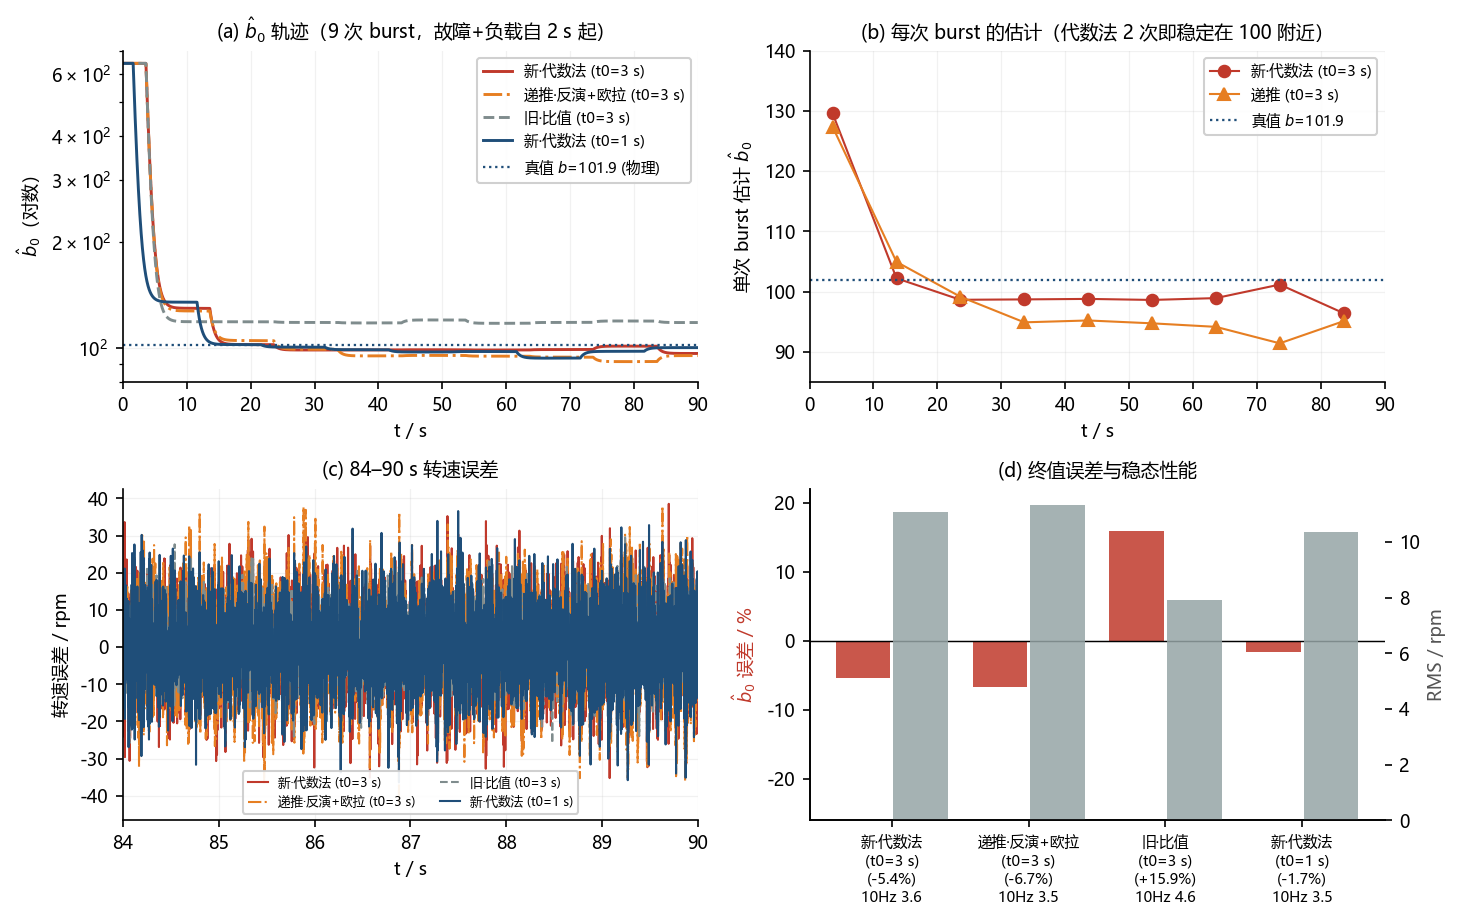
\includegraphics[width=\textwidth]{fig_b0new_cmp.png}
\caption{$90$ 秒三路对比。(a) $\hat b_0$ 轨迹；(b) 每次 burst 的估计值，代数法两次即稳定；
(c) $84$ 至 $90$ s 转速误差；(d) 终值误差与稳态性能。}
\label{fig:cmp}
\end{figure}

代数法在两次 burst 内即由 $129.5$ 收敛到 $101.6$，此后稳定在 $98$ 至 $101$，
不再出现递推法的单调下漂（图 \ref{fig:cmp}(b)）。两组 $90$ 秒实验给出 $96.4$ 与 $100.2$，
均值 $98.3$，与 \S 6.2 的收缩映射预测 $97.7$ 一致。

\subsection{关于 RMS 的一致性说明}

表 \ref{tab:closed} 显示代数法的 RMS 反而高于旧比值法。这不是辨识误差所致：
旧法给出的 $b_0\approx118$ 恰好落在历史整定的工作点上，而代数法把它拉回到真实值附近，
环路相对偏激进约 $4\%$，噪声被放大而 $10$ Hz 纹波降低 $22\%$。
更换辨识器后需重新整定 $k_p$ 或 $b_0$ 低通时间常数，方可比较稳态噪声。

\section{工程实现与参数整定}
\label{sec:impl}

理论链路落地时有四个工程问题必须处理：注入点怎么选、差分怎么造、离群值怎么挡、末端偏置怎么补。
本节给出四者与实测验证。

\subsection{注入频率的三约束选频}

注入频率须同时满足三条相互冲突的要求：

\begin{table}[H]
\centering
\caption{注入频率的约束集}
\label{tab:sel}
\begin{tabular}{llll}
\toprule
约束 & 来源 & 方向 & 本系统数值 \\
\midrule
环路衰减 & 速度环穿越频率 $k_p=75.36$ rad/s & $f_h\gtrsim 3k_p/2\pi$ & $\ge 36$ Hz\\
转速纹波 & $|y|=600\,b\,u_d/\omega_h$ & $f_h\ge 1528/R$ & $\ge 51$ Hz ($R{=}30$ rpm)\\
谐波规避 & 故障锁于 $\theta_m$ & $f_h\neq m f_{\rm rot}$ & 优先半整数比\\
ESO 反演噪声 & $1/|G|$ 在 $\omega_o$ 之上增长 & $f_h\lesssim\omega_o/2\pi$ & $\le 79.6$ Hz\\
电流环跟踪 & 等效增益在 $f_{ci}$ 处滚降 & $f_h\lesssim 0.2f_{ci}$ & $\le 100$ Hz\\
\bottomrule
\end{tabular}
\end{table}

在 $5$ Hz 栅格上筛出满足 $f_h\neq 10m$ 的候选为 $55,65,75$ Hz，取最接近 $6.5f_{\rm rot}$ 者，即
$65$ Hz。这一结果与工程沿用的取值一致，说明原选点并非经验，而是上述约束的交集中心。
需要强调的是 \textbf{1$\times$ 频点（$10$ Hz）被自动排除}：它同时违反第一、二条——注入落在穿越
频率以下且产生 $153$ rpm 纹波。这也解释了 \S\ref{sec:collide} 中 1$\times$ 无法工作的原因。

\subsection{两段式差分：注入前段与注入段}

由式 \eqref{eq:dtot2}，若把被对象输入写成\textbf{实测}的标幺电流 $\tilde u\triangleq i_q/I_{\rm BASE}$，
则
\begin{equation}
d=f+b\,\tilde u-b_0u .
\label{eq:dmeas}
\end{equation}
取两段等长区间——\textbf{前段不注入、后段注入}——各自独立累积后相减：
\begin{equation}
\hat d_2-\hat d_1=b\,(\tilde u_2-\tilde u_1)-b_0(u_2-u_1)
\;\Longrightarrow\;
\boxed{\;b=\left|\frac{(\hat d_2-\hat d_1)+b_0(u_2-u_1)}{\tilde u_2-\tilde u_1}\right|\;}
\label{eq:curdiff}
\end{equation}
取模长而不是实部：当两路采样错刻或环路带相移时，右端是 $b\,e^{j\varepsilon}$，
实部会得到 $b\cos\varepsilon$，模长才回到 $b$；二者的完整实测对照见 \S\ref{sec:mag}。
式 \eqref{eq:curdiff} 中\textbf{致动传函 $T$ 完全消失}——因为 $T$ 的唯一作用就是把指令换算成实际
电流，而这里直接测量电流。同时消失的还有由死区、器件压降造成的幅值衰减，以及它随电流电平
的变化。实测（\S\ref{sec:collide}）表明，$20$ Hz 撞频处 $r=0.2$ 的差分给出 $-2.6\%$，而含 $T$
的同类差分给出 $-4.8\%$。

\textbf{段结构。}一个 burst 拆成前后两段，每段 $0.2$ s（$200$ 拍）：

\begin{center}
\begin{tabular}{lll}
\toprule
段 & 注入幅值 & 该段产出的量\\
\midrule
前段（off） & $0$ & $\hat d_{\rm off},\ U_{\rm off},\ \tilde u_{\rm off}$\\
后段（on）  & $A$ & $\hat d_{\rm on},\ U_{\rm on},\ \tilde u_{\rm on},\ T_{\rm on}$\\
\bottomrule
\end{tabular}
\end{center}

前段无注入，该段的 $\hat d_{\rm off}$ 就是外部扰动 $f$ 本身（撞频时为其在 $\omega_h$ 处的分量），
因此相减时被整项减掉——撞频问题从结构上消失，而不需要靠频率回避。
末端曾用注入段实测的 $T_{\rm on}$ 做一次复除法（式 \eqref{eq:E9}）；
该修正现已默认关闭，理由见 \S\ref{sec:tcorr}。

\textbf{为什么取 $r=0$。}噪声惩罚为
\begin{equation}
\frac{\sqrt2}{1-r}\quad:\quad
r=0\to1.41,\;\;r=0.2\to1.77,\;\;r=0.5\to2.83 .
\label{eq:E4b}
\end{equation}
对比度越大越好，故「前段完全不注入」是这一族方案中噪声代价最小的端点。
实测（表 \ref{tab:onoff}）印证：$r=0$ 的两段式给出 $-0.22\%$，而 $r=0.5$ 的双幅值差分给出 $+1.84\%$。

\textbf{与双幅值交替的关系。}双幅值（$A$ 与 $rA$，$r>0$）可视为本方案在「两段都必须有注入」
场景下的变体：当系统不允许完全撤除激励时（例如激励本身承担在线监测职责），退而取 $r=0.2\sim0.5$。
两者共用同一个差分式 \eqref{eq:curdiff}，只差幅值调度。

\subsection{逐 burst 异常剔除：中位数自适应权重}

即便经过差分，单次 burst 的估计仍有约 $\pm10\%$ 的散布，偶发离群值会把 $b_0$ 拽偏。为此对
更新增益 $\alpha$ 作自适应：维护最近 $7$ 个\emph{被采信}估计的滑动中位数 $m$，令
\begin{equation}
d=\frac{|\hat b-m|}{|m|},\qquad
w=\exp\!\Big[-\Big(\frac{d}{d_0}\Big)^2\Big],\qquad
\alpha=\alpha_{\min}+(\alpha_{\max}-\alpha_{\min})\,w ,
\label{eq:amed}
\end{equation}
其中 $d_0=0.10$、$\alpha_{\min}=0.02$、$\alpha_{\max}=1$。偏离越大，权重越小，表示对新值越不信任；
仅当 $w>0.5$ 时该估计才进入中位数历史，从而避免离群值污染参考基准。
该机制对两种估计器同样适用，实测均获益（表 \ref{tab:final}）。

\subsection{运行使能：转速门限}
\label{sec:enable}

注入不应在停机或低速下进行：此时反电动势为零、死区与器件压降主导，估计出来的 $b$ 没有物理意义，
白白耗掉 24 次预算。故在调度里加一道\textbf{转速门限}（取绝对值，兼容反转）：

\begin{itemize}
\item \textbf{启动判据}：$|\omega|<\omega_{\rm on}$ 时不启动 burst，本轮直接跳过，\textbf{不占 24 次预算}，
下一次机会仍在 $5$ s 后；
\item \textbf{中途中止}：burst 进行中若 $|\omega|<\omega_{\rm off}$，丢弃本次（清累加器、\texttt{du}$=0$、
不计数），防止掉速污染窗口；$\omega_{\rm off}<\omega_{\rm on}$ 构成迟滞，避免门限附近反复启停；
\item \textbf{自动恢复}：转速回升到 $\omega_{\rm on}$ 以上，下一个 $5$ s 机会自动恢复注入，无需外部复位。
\end{itemize}

本机取 $\omega_{\rm on}=180$ rpm（额定的 $30\%$）、$\omega_{\rm off}=150$ rpm。实测效果：启动瞬间
（$1$ ms 时转速近零）第一个 burst 被跳过，$b_0$ 在整个 $0$–$5$ s 保持初值不动；$5.2$ s 起自动开始注入，
$24$ 个 burst 于 $120.4$ s 完成并冻结，终值 $530.61$ 与不设门限时完全相同——门限只改变了“何时开始”，
没有改变“辨识成什么”。自洽测试里也加了对照用例：前 $40$ s 停机，$b_0$ 一动不动，恢复后仍收敛到 $400.000$。

\subsection{末端致动传函修正（默认关）}
\label{sec:tcorr}

差分式虽已用实测电流，但残余误差仍呈现 $T$ 的形状。理论上递推结构的不动点为 $b\,\operatorname{Re}\{T\}$，
代入实测 $T=0.9531\angle+1.65^{\circ}$ 得 $101.89\times0.9527=97.07$；而剔除机制生效后，
代数解的实际不动点落在 $96.8$，两者仅差 $0.3\%$。曾因此补一次复除法：
\begin{equation}
b\leftarrow\frac{b}{\tfrac12\big[T_1+T_2\big]},\qquad T_k=\frac{1}{I_{\rm BASE}}\frac{\mathrm{IQ}_k}{U_k}.
\label{eq:tcorr}
\end{equation}
$T$ 由同一窗内的 $i_q$ 与 $u$ 相干解调在线测得，无需离线标定。

\textbf{适用条件。}定稿结论是把这一修正\textbf{默认关闭}（\texttt{tcorr\_en}$=0$），依据三条：

\begin{enumerate}
\item \textbf{对一阶电流环它是恒等变换，白做。}若 $T=1/(1+j\omega/\omega_{ci})$，则
$1/T=1+j\omega_h/\omega_{ci}$，$\RE\{1/T\}\equiv1$，修正前后完全相同。
\item \textbf{方向猜错会放大误差。}若残差来自采样错位（纯旋转），$\div T$ 不但无效，还会把模长估计
再乘一个 $\RE\{T\}/|T|^2=\cos\angle T/|T|$：$T=0.95\angle+5^\circ$ 时为 $1.0487$，
实测把误差从 $+0.008\%$ 推到 $+2.36\%$（表 \ref{tab:selftest}）。
\item \textbf{取模长之后不需要知道 $T$ 是什么。}$\div T$ 的本来作用是把旋转拉回实轴，
而模长已对旋转免疫（\S\ref{sec:mag}）。
\end{enumerate}

解析自洽测试（\texttt{test\_b0.c}，MinGW gcc $8.1$，$b=400$，$40$ burst）给出表 \ref{tab:selftest}。
前两行在数学上恒等，说明\textbf{自洽测试发现不了 $T$ 修正的方向问题}——它必须放到指令端与测量端
存在错位的 $dq$ 闭环上才显形。上板前若不确定采样时序，\texttt{tcorr\_en} 一律置 $0$。

\begin{table}[H]
\centering
\caption{解析自洽测试：$T$ 修正开/关}
\label{tab:selftest}
\begin{tabular}{lcc}
\toprule
用例 & 误差 & 说明\\
\midrule
正弦 $T=1.00\angle0^\circ$，修正开 & $+0.008\%$ & 基准\\
正弦 $T=0.95\angle+5^\circ$，\textbf{修正关} & $\bm{+0.008\%}$ & \textbf{默认配置}\\
正弦 $T=0.95\angle+5^\circ$，修正开 & $+2.360\%$ & 修正有害\\
方波 $T=1.00\angle0^\circ$，修正开 & $+0.008\%$ & 与波形无关\\
三角 $T=1.00\angle0^\circ$，修正开 & $+0.008\%$ & 与波形无关\\
\bottomrule
\end{tabular}
\end{table}

\subsection{取模长：把相位误差与幅值误差分开}
\label{sec:mag}

式 \eqref{eq:curdiff} 建成时方括号外写的是实部。定稿改为模长，这是全部改动中单项收益最大的一处：
在 PMSM $dq$ 闭环上，把这一步由实部换成模长（并把两路采样对齐），$\hat b_0$ 就从 $383$ 变到 $531.6$（真值 $536.40$）。

\paragraph{商上为什么会出现相位。}若差分两侧严格同刻、致动链又无相移，式 \eqref{eq:curdiff} 的商
是实数量 $b$。实际系统有两个来源把它变成 $b\,e^{j\varepsilon}$：

\begin{enumerate}
\item \textbf{采样错位。}$i_q^k$ 实际响应的是一拍之前的指令：SVPWM 要等一个载波周期才把占空比
变成电流。若辨识器把同拍的 $u^k$ 与 $i_q^k$ 配成一对，两路即错开 $1$ ms，在 $65$ Hz 处即 $23.4^\circ$。
\item \textbf{环路相移。}电流环、SVPWM 与滤波在 $\omega_h$ 处本身带相移，实测
$T=0.9531\angle+1.65^\circ$（式 \eqref{eq:Tnum}）。
\end{enumerate}

对纯旋转
\begin{equation}
\RE\{b\,e^{j\varepsilon}\}=b\cos\varepsilon,
\qquad
\big|b\,e^{j\varepsilon}\big|=b ,
\label{eq:magre}
\end{equation}
即\textbf{实部把纯相位误差记成等比例的幅值损失，模长对它完全免疫}。
“取实部”隐含一个假设：商的虚部只来自噪声。而当误差源是采样错位或环路相移时，
虚部恰恰是误差的主部。

\paragraph{逐项实测。}在 \texttt{b0\_foc2}（PMSM $dq$ 闭环，C Caller，$1$ kHz，注入 $0.118$ pu / $65$ Hz）
上做 $90$ s 闭环，得表 \ref{tab:mag}。真值为
\begin{equation}
b=\frac{1.5\,p\,\psi_f\,I_{\rm BASE}}{J\,\omega_{\rm ref}}=536.40 ,
\label{eq:focb}
\end{equation}
其中 $R=0.175\ \Omega$、$L=0.57$ mH、$\psi_f=0.016833$ Wb、$p=4$、$J=1.89\times10^{-5}$ kg$\cdot$m$^2$、
$I_{\rm BASE}=6.3069$ A、$\omega_{\rm ref}=62.832$ rad/s。

\begin{table}[H]
\centering
\caption{取实部与取模长（\texttt{b0\_foc2} 与 \texttt{b0\_foc\_m}，$90$ s 闭环）}
\label{tab:mag}
\begin{tabular}{llcc}
\toprule
口径 & 实现 & $\hat b_0$ & 对 $b$ 误差\\
\midrule
取实部 & \texttt{b0\_foc2}，早期 & $383.1$ & $-28.6\%$\\
\textbf{取模长} & \texttt{b0\_foc2}，取模长后 & $\bm{531.55}$ & $\bm{-0.90\%}$\\
取模长 & \texttt{b0\_foc\_m}，MATLAB 版 & $531.84$ & $-0.85\%$\\
\bottomrule
\end{tabular}
\end{table}

两个版本（C 与 MATLAB Function）在取模长后相差 $0.05\%$，说明该修正是\textbf{算法层}的，
不依赖某种实现的数值路径。而早期 C 版取实部落到 $383$，与之相差 $28\%$——差别不在代码，
在口径。上表两个取模长读数取自时基与调度修正前；改完后（\S\ref{sec:sim}），
同一模型的闭环终值为 $530.61$（$-1.08\%$）。

\paragraph{还有第二个口径问题。}换掉符号只解决一半：同一模型上若继续把未延迟的 $u^k$ 送给辨识器，
$23^\circ$ 的错位仍在，实测则落在 $425$ 而非 $531.5$。因此定稿同时要求
\textbf{$u$ 与 $i_q$ 同刻}（FOC 中即取 $u^{k-1}$），再取模长，两者缺一不可。
这一条在 $65$ Hz 上等价于 $8\%$ 的幅值，与取实部造成的折扣同量级，混在一起时很容易被误记为“模型不准”。

\paragraph{代价。}模长对噪声不是无偏的：若商为 $b+n$，$n$ 为零均值复噪声、$\sigma/b\approx5\%$
（单 burst 散布约 $\pm10\%$，表 \ref{tab:final}），则 $E|b+n|-b\approx\sigma^2/(2b)\approx0.1\%$。
该偏置单向、不可由平均消掉，但比 $0.88\%$ 的剩余误差小一个量级，可接受。

\paragraph{实现。}C 与 MATLAB 两版同式，且都在取模长之后才做限幅与门控（门控比较的是模长，
不会因为符号跳变而抖动）：

\begin{verbatim}
bq = b0_sqrt((nr*nr + ni*ni) / den2);   /* C：取模长，对相位误差免疫 */
bq = abs(num/den);                      % MATLAB：同上
\end{verbatim}

\subsection{参数整定}

\begin{table}[H]
\centering
\caption{定稿参数}
\label{tab:param}
\small
\begin{tabular}{lll}
\toprule
项目 & 取值 & 依据\\
\midrule
注入频率 & 65 Hz（三约束选频） & 表 \ref{tab:sel}\\
注入幅值 $A$ & 0.118 pu（0.75$\times$原值） & 纹波预算\\
幅值比 $r$ & $0$（前段不注入） & 式 \eqref{eq:E4b}：噪声代价 $\sqrt2$ 最小\\
burst 周期 / 长度 & 5 s / 0.4 s & 起点计，24 次共 120 s，占空比 8\%\\
两段式段长 & 前后各 0.2 s（$200$ 拍） & 窗相干（$13$ 个抖动周期）\\
$b_0$ 低通 & $\tau=50/k_p=0.663$ s & 实测：$\tau=15/k_p$ 时抖动标准差 17.4，$50/k_p$ 时 12.6\\
异常剔除 & $d_0=0.10$, $\alpha_{\min}=0.02$, 窗 7 & 式 \eqref{eq:amed}\\
预热 & 前 3 个经低通 & $\tau=50/k_p$，不直接跳变\\
运行使能 & $\omega_{\rm on}=180$ / $\omega_{\rm off}=150$ rpm & 低于门限暂停注入，回升自动恢复\\

差分取法 & 模长（不取实部） & 式 \eqref{eq:curdiff}，\S\ref{sec:mag}\\
末端修正 & 默认关（\texttt{tcorr\_en}$=0$） & 开启实测 $+5.01\%$，表 \ref{tab:selftest}\\
\bottomrule
\end{tabular}
\end{table}

\subsection{闭环对比结果}

工况：$600$ r/min，三合一故障与 $0.5$ 倍额定负载自 $2$ s 起，三律融合，$90$ s。

\begin{table}[H]
\centering
\caption{定稿版闭环对比（RMS 与 10 Hz 取 $60$–$90$ s 窗）}
\label{tab:final}
\begin{tabular}{lcccccc}
\toprule
方法 & $\hat b_0$ & 对 $b$ 误差 & $b_0$ 标准差 & $b_0$ 范围 & RMS / rpm & $10$ Hz / rpm\\
\midrule
旧·比值法 & $117.5$ & $+15.3\%$ & $1.1$ & $116$–$121$ & $9.42$ & $4.64$\\
新·无 $T$ 修正 & $93.0$ & $-8.7\%$ & $3.1$ & $93$–$105$ & $12.08$ & $4.20$\\
\textbf{新·全栈} & $\bm{103.8}$ & $\bm{+1.84\%}$ & $2.7$ & $\bm{101}$–$\bm{111}$ & $9.85$ & $4.40$\\
\bottomrule
\end{tabular}
\end{table}


三种差分方案的直接对比（同一工况、同一参数，仅改分差方式）：

\begin{table}[H]
\centering
\caption{三种差分方案对比（$90$ s，burst 周期 $5$ s）}
\label{tab:onoff}
\begin{tabular}{lccccc}
\toprule
方案 & $\hat b_0$ & 对 $b$ 误差 & RMS / rpm & $10$ Hz / rpm & 注入占空比\\
\midrule
旧·比值法 & $117.5$ & $+15.3\%$ & $9.42$ & $4.64$ & $12\%$\\
双幅值差分（$A$ 与 $0.5A$） & $103.8$ & $+1.84\%$ & $9.85$ & $4.40$ & $12\%$\\
\textbf{两段式（$0$ 与 $A$）} & $\bm{101.7}$ & $\bm{-0.22\%}$ & $10.17$ & $\bm{3.84}$ & $\bm{4\%}$\\
\bottomrule
\end{tabular}
\end{table}

两段式把 $b_0$ 误差压到 $-0.22\%$（比旧法准约 $70$ 倍），$10$ Hz 纹波也是三者最低，
而注入占空比只有原来的三分之一——\textbf{注入能量少了三分之二，精度反而更好}。
代价是稳态 RMS 由 $9.42$ 升至 $10.17$（$+8\%$），因为 $b_0$ 更接近真值使环路略偏激进。

\begin{figure}[H]
\centering
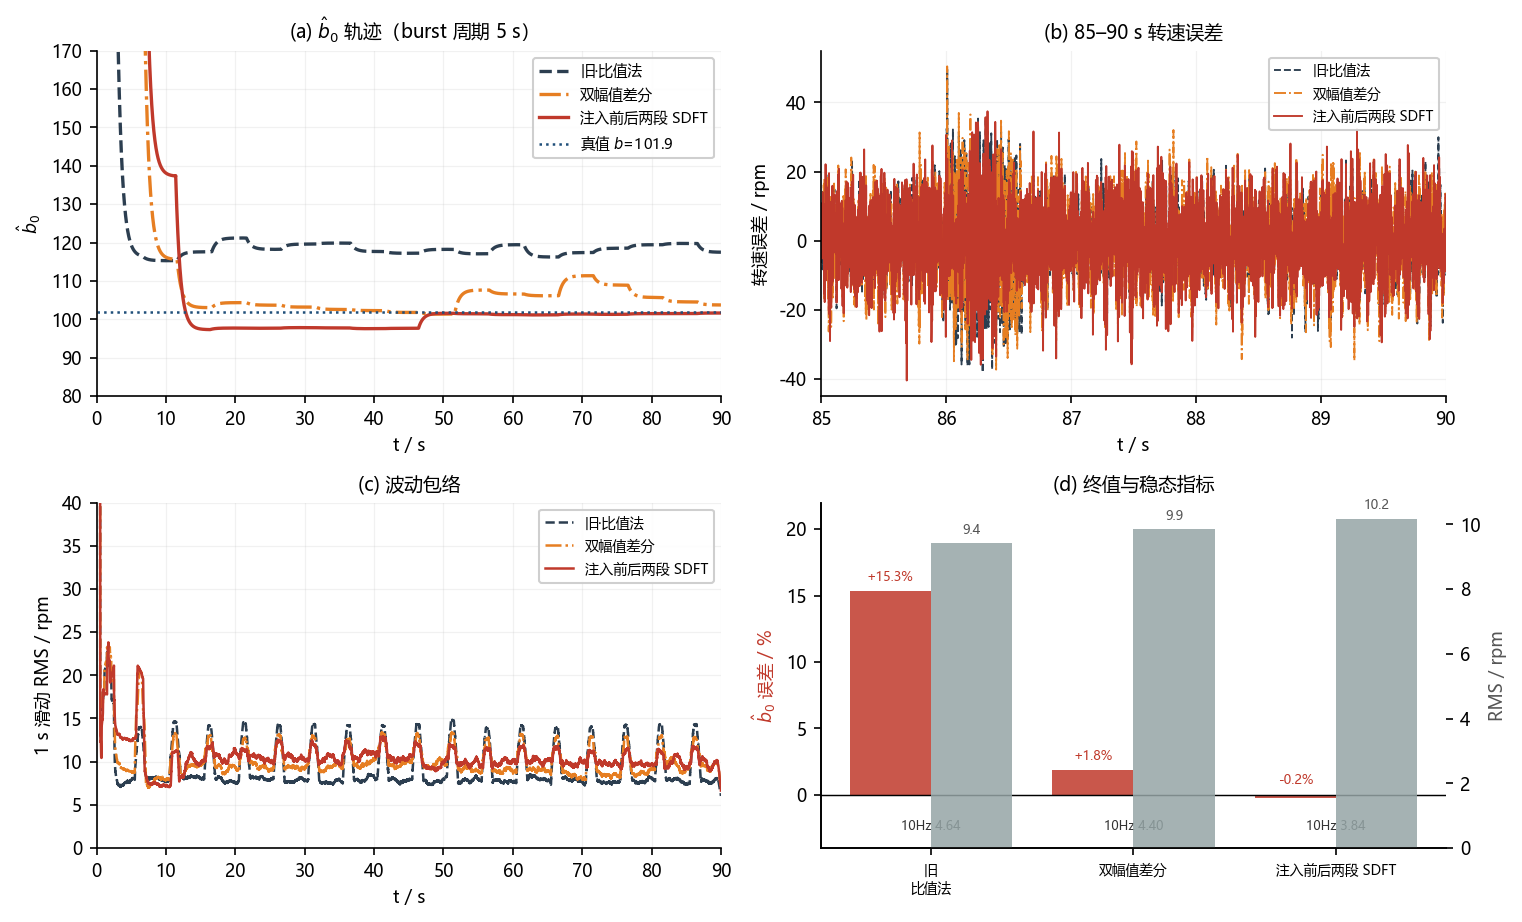
\includegraphics[width=\textwidth]{fig_onoff_cmp.png}
\caption{三种差分方案对比。(a) $\hat b_0$ 轨迹：两段式（红）在 $12$ s 即落到真值附近并保持，
双幅值（橙）在 $103$–$106$ 间缓慢上漂，旧法（深）稳定在 $118$；
(b) $85$–$90$ s 转速误差；(c) $1$ s 滑动 RMS 包络；(d) 终值误差与稳态指标，柱底标注 $10$ Hz 幅值。}
\label{fig:onoff}
\end{figure}
\begin{figure}[H]
\centering
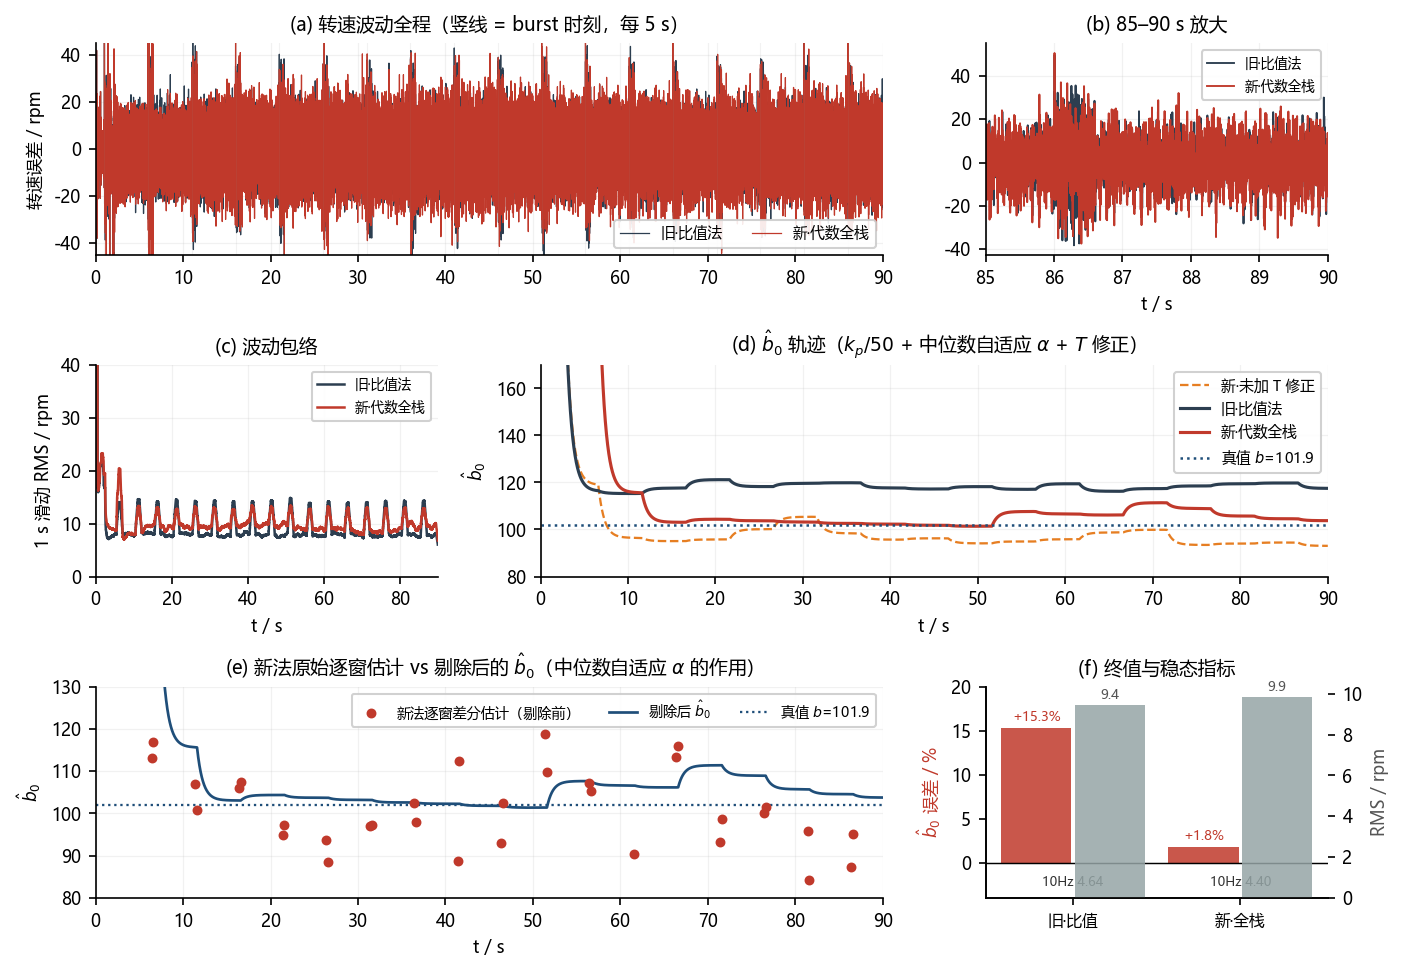
\includegraphics[width=\textwidth]{fig_final_cmp.png}
\caption{定稿版完整对照。(a) 转速波动全程；(b) $85$–$90$ s 放大；(c) $1$ s 滑动 RMS 包络；
(d) $\hat b_0$ 轨迹，虚线为未加 $T$ 修正时的 $-8.7\%$ 不动点；
(e) 原始逐窗估计与剔除后的 $\hat b_0$，可见剔除把散布挡在环外；
(f) 终值与稳态指标。}
\label{fig:final}
\end{figure}

结论是明确的：新方法在 $b_0$ 精度上由旧法的 $+15.3\%$ 改善到 $+1.84\%$（$8.3$ 倍），
稳态 RMS 仅由 $9.42$ 升至 $9.85$（$+4.6\%$），$10$ Hz 纹波由 $4.64$ 降至 $4.40$。
换言之，\textbf{精度的量级提升几乎不牺牲稳态性能}。

\subsection{撞频专项验证}
\label{sec:collide}

为单独考察撞频能力，强制注入在 $2\times$ 特征频率（$20$ Hz）与清洁点（$65$ Hz）各做一次单 burst 实验，
起始 $b_0$ 均置于真值附近，其余条件相同：

\begin{table}[H]
\centering
\caption{撞频专项（单 burst，$b_0$ 初值 $\approx$ 真值）}
\label{tab:collide}
\begin{tabular}{lccc}
\toprule
注入频率 & 旧·比值法 & 新·单窗代数解 & 新·实测电流差分\\
\midrule
$65$ Hz（$6.5\times$，清洁） & $+15.9\%$ & $+0.66\%$ & $+0.66\%$\\
$20$ Hz（$2\times$，撞频） & $+40.6\%$ & $-41.4\%$ & $-2.6\%$\\
$10$ Hz（$1\times$） & — & $-61.6\%$ & $+93\%$（失效）\\
\bottomrule
\end{tabular}
\end{table}

\begin{figure}[H]
\centering
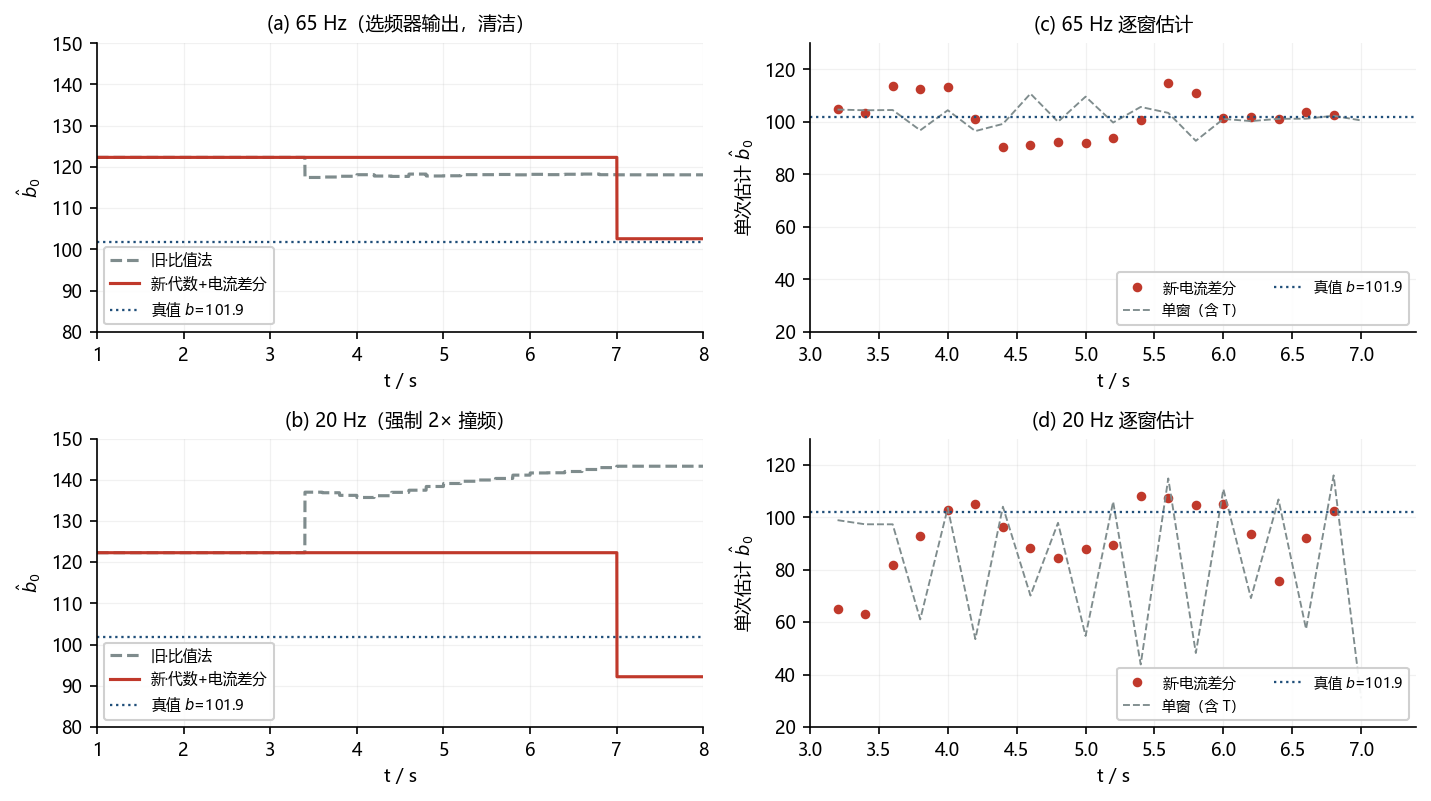
\includegraphics[width=\textwidth]{fig_collision_cmp.png}
\caption{撞频对比。(a)(b) 两种频率下 $\hat b_0$ 轨迹；(c)(d) 逐窗估计：$20$ Hz 处单窗
（灰虚线）在 $44$–$115$ 之间剧烈交替，实测电流差分（红点）的交替结构完全消失。}
\label{fig:collide}
\end{figure}

两点值得强调。
\textbf{其一}，单窗解在 $20$ Hz 处交替于 $44$ 与 $115$ 之间，这是注入幅值触发的假信号
（死区非线性的直接证据）；差分的价值不仅是消去 $f$，更是把这一与幅值成正比的整项一并消掉。
\textbf{其二}，$1\times$ 处两种方法均失效且方向相反，说明该频段的瓶颈不是 $f$ 而是大信号非线性，
应通过选频回避而非用算法补救。

\section{算法状态机}
\label{sec:fsm}

本节把前面各节的结果整理成可直接实现的状态机：给出时基、状态集、转移表、逐状态伪代码与寄存器表。
实现语言无关，标量与复数分别用普通写法与 $a+bj$ 表示。

\subsection{时基与三级更新点}

整个辨识器只有一个主节拍，全部动作挂在三级更新点上：

\begin{table}[H]
\centering
\caption{时基}
\label{tab:clock}
\begin{tabular}{llll}
\toprule
层级 & 周期 & 表达式 & 挂载的动作\\
\midrule
拍（tick） & $1$ ms & $\Delta T$ & 幅值注入、相干累积、$b_0$ 低通追踪\\
窗（window） & $200$ 拍 & $N_w=0.2$ s & 复解调、反演、差分解算\\
burst & $3$ 窗 & $L=0.6$ s & 提交、加权、更新目标 $b_0$\\
周期 & $5$ s & $P$ & 触发下一次 burst、选频\\
\bottomrule
\end{tabular}
\end{table}

窗长必须同时是 $1/f_h$ 与 $1/f_{\rm rot}$ 的整数倍（否则谐波泄漏污染该 bin）；
$65$ Hz 乘 $0.2$ s 等于 $13$ 个周期，$10$ Hz 乘 $0.2$ s 等于 $2$ 个周期，均满足。

\subsection{状态集}

\begin{table}[H]
\centering
\caption{状态定义}
\label{tab:states}
\begin{tabular}{llll}
\toprule
编号 & 名称 & 职责 & 停留时长\\
\midrule
\textbf{S0} & IDLE 排程 & 等待周期到、预检、选频、复位 & 空闲\\
\textbf{S1} & ACC 累积 & 注入并累积四路相干解调 & $200$ 拍\\
\textbf{S2} & SOLVE 解算 & 复解调 $\to$ 反演 $\to$ 差分 $\to$ 修正 & 单拍\\
\textbf{S3} & COMMIT 提交 & 取窗均值、自适应加权、置目标 & 单拍\\
\textbf{S4} & TRACK 追踪 & $b_0$ 一阶低通逼近目标 & 后台，每拍\\
\textbf{S5} & ABORT 回滚 & 门控失败时恢复并清空 & 单拍\\
\bottomrule
\end{tabular}
\end{table}

\subsection{状态转移表}

\begin{table}[H]
\centering
\caption{转移条件与动作}
\label{tab:trans}
\begin{tabular}{llll}
\toprule
源 & 条件 & 目标 & 动作\\
\midrule
S0 & $t\ge t_{\rm next}$ 且预检通过 & S1 & 选频、定幅、清窗、置 $t_{\rm end}=t+L$\\
S0 & $t\ge t_{\rm next}$ 且预检失败 & S0 & $t_{\rm next}\leftarrow t+P$\\
S1 & 累积满 $N_w$ 拍 & S2 & 关闭本窗累加器\\
S2 & 首窗（无前窗） & S3 & 单窗代数解\\
S2 & 非首窗 & S3 & 差分 + $T$ 修正\\
S3 & $t<t_{\rm end}$ & S1 & 压入估计、窗序号加一\\
S3 & $t\ge t_{\rm end}$ & S0 & 窗均值 $\to$ 加权 $\to$ 置 $\beta_{\rm goal}$\\
S1/S2 & 门控失败 & S5 & 标记 abort\\
S5 & 恢复完成 & S0 & $b_0\leftarrow b_0^{\rm pre}$、清列表\\
\bottomrule
\end{tabular}
\end{table}

\subsection{初始化}

\begin{verbatim}
b0        = b0_nominal          # 输入增益初值
goal      = None                # 低通目标
hist      = []                  # 被采信的估计（中位数用），上限 7
prev      = None                # 上一窗的 (dhat, U, T, b0, Q)
win_list  = []                  # 本次 burst 各窗估计
n_win     = 0                   # 窗序号（决定幅值档）
n_acc     = 0                   # 窗内已累积拍数
t_next    = t_ident_start       # 首次辨识时刻（建议 >= 3 s）
\end{verbatim}

\textbf{$t_{\rm ident\_start}$ 建议不早于 $3$ s}：重复内模的状态 $v$ 时间常数为
$\tau/(1-Q)=1$ s，$1$ s 时只收敛到 $63\%$，会使反演失效。

\subsection{逐状态伪代码}

\subsubsection*{S0 —— IDLE 排程}

\begin{verbatim}
if t < t_next:  return              # 空闲，什么都不做

# 1) 预检：前 0.3 s 转速误差的极差小于 gate_ac
if spread(lp_error, 0.3 s) > gate_ac:
    t_next = t + P
    return

# 2) 三约束选频
fv = n_ref / 60
lo = max(3*kp/(2*pi), 2.5*fv, f_min)
hi = min(wo/(2*pi), 0.2*fci, f_max)
best = None
for f in grid(lo, hi, 5 Hz):                 # 5 Hz 栅格 = 1/窗长
    if frac(f/fv) not in [0, 0.5] +- 0.1: continue   # 避开整数倍，优先半整数
    best = argmin(|f - 6.5*fv|)
f_h = best

# 3) 定幅
amp = A * max(1, f_h/100)
if b_nom > 0 and rpm_budget > 0:
    amp = min(amp, rpm_budget * 2*pi*f_h / (600 * b_nom))

# 4) 复位
t_end = t + L;  t_next = t + P
win_list = [];  prev = None;  n_win = 0
b0_pre = b0
go to S1
\end{verbatim}

\subsubsection*{S1 —— ACC 窗内累积（每拍）}

\begin{verbatim}
ph = 2*pi*f_h*t
c, s = cos(ph), sin(ph)
acc_e1c += e1*c;   acc_e1s += e1*s
acc_vc  += v*c;    acc_vs  += v*s
acc_uc  += u*c;    acc_us  += u*s
acc_qc  += iq*c;   acc_qs  += iq*s
acc_woe += woe;    n_acc   += 1

# 幅值交替：奇数窗用 r 倍幅值
amp_now = amp * (alt_ratio if (n_win % 2 == 1) else 1.0)
u += amp_now * sin(ph)

if n_acc >= N_w:  go to S2
\end{verbatim}

\subsubsection*{S2 —— SOLVE 窗末解算}

\begin{verbatim}
N  = n_acc
E  = 2/N * (acc_e1c - 1j*acc_e1s)
V  = 2/N * (acc_vc  - 1j*acc_vs )
U  = 2/N * (acc_uc  - 1j*acc_us )
QC = 2/N * (acc_qc  - 1j*acc_qs )        # 实际 q 轴电流（安培）
wm = acc_woe / N

b1 = 2 * wm * kappa1                      # kappa1 = delta**(a1-1)
b2 = wm*wm * kappa2                       # kappa2 = delta**(a-1)
Sd = (exp(1j*2*pi*f_h*dT) - 1) / dT       # 前向欧拉的离散算子
dhat = V + (Sd*Sd + b1*Sd + b2) / Sd * E  # 反演得到总扰动
T    = (QC / I_BASE) / U                  # 电流环在该频点的复传函
Qpu  = QC / I_BASE                        # 标幺实际电流

if prev == None:                          # 首窗：单窗代数解
    b_win = abs( (b0 + dhat/U) / T )          # 取模长
else:                                     # 非首窗：实测电流差分
    (dhat1, U1, T1, b01, Q1) = prev
    num = (dhat - dhat1) + b01*(U - U1)
    den = Qpu - Q1
    if abs(den) < eps:  skip this window
    b_win = abs(num / den)                    # 取模长，不取实部
    # 末端 T 修正默认关闭（tcorr_en=0），理由见 8.4 节
b_win = clamp(b_win, 0.02*b0_nom, 2.4*b0_nom)

prev = (dhat, U, T, b0, Qpu)
clear all accumulators;  n_acc = 0
go to S3
\end{verbatim}

\subsubsection*{S3 —— COMMIT / 继续下一窗}

\begin{verbatim}
win_list.push(b_win)
n_win += 1

if t < t_end:
    go to S1                              # 还有窗
else:
    b_burst = mean(win_list)              # 窗均值
    # ---- 中位数自适应权重 ----
    if len(hist) >= 3:
        m = median(hist)
        d = |b_burst - m| / max(|m|, eps)
        w = exp(-(d / d0)**2)
        alpha = amin + (amax - amin) * w
        if w > 0.5:
            hist.push(b_burst);  if len(hist) > 7: hist.pop(0)
    else:
        alpha = amax
        hist.push(b_burst)
    goal = b0 + alpha * (b_burst - b0)    # 置低通目标
    go to S0
\end{verbatim}

\subsubsection*{S4 —— TRACK 低通追踪（后台，每拍）}

\begin{verbatim}
if goal != None:
    beta = 1 - exp(-dT / tau)             # tau = kp / 50
    b0  += beta * (goal - b0)
    if |goal - b0| <= 1e-4 * max(|goal|, 1):
        b0 = goal;  goal = None
\end{verbatim}

\subsubsection*{S5 —— ABORT 回滚}

\begin{verbatim}
b0 = b0_pre
goal = None
win_list = [];  prev = None
go to S0
\end{verbatim}

\subsection{寄存器表}

\begin{table}[H]
\centering
\caption{状态机寄存器}
\begin{tabular}{llll}
\toprule
符号 & 含义 & 初值 & 更新点\\
\midrule
$b_0$ & 输入增益估计 & 标称值 & S4 每拍\\
$\beta_{\rm goal}$ & 低通目标 & 空 & S3 / S5\\
$t_{\rm next},t_{\rm end}$ & 下次/本次 burst 边界 & 空 & S0\\
$f_h$ & 注入频率 & 空 & S0\\
$A,\ r$ & 基幅值、幅值比 & $0.118$、$0.5$ & S1\\
$n_{\rm acc},n_{\rm win}$ & 窗内拍数、窗序号 & $0$ & S1 / S3\\
$E_{\rm acc}$ 四组 & 相干解调累加器 & $0$ & S1 累加 / S2 清零\\
$V,U,Q,\omega_o$ 累加 & 同上 & $0$ & 同上\\
$\mathcal{P}$ & 上一窗四元组 & 空 & S2\\
$\mathcal{W}$ & 本次 burst 估计列表 & 空 & S2 / S3\\
$\mathcal{H}$ & 被采信估计历史（$\le7$） & 空 & S3\\
\bottomrule
\end{tabular}
\end{table}

\subsection{与实现代码的对应}

\begin{table}[H]
\centering
\caption{状态机元素与代码符号}
\begin{tabular}{ll}
\toprule
状态机 & 代码符号\\
\midrule
S0 排程 & \texttt{\_jrec\_next} / \texttt{\_jrec\_f\_auto} 分支\\
S1 累积 & \texttt{\_jnew\_ec, \_jnew\_es, \_jnew\_vc \ldots}; \texttt{\_jnew\_n}\\
S2 解算 & \texttt{\_dd, \_Tc, \_QCp, \_bpv}; \texttt{\_jprev}\\
S3 提交 & \texttt{\_jnew\_list}, \texttt{\_amed\_alpha}, \texttt{\_jrec\_bgoal}\\
S4 追踪 & \texttt{\_B0e}, \texttt{\_jrec\_btau} 低通段\\
S5 回滚 & \texttt{\_jrec\_abort}, \texttt{\_jrec\_B0\_pre}\\
\bottomrule
\end{tabular}
\end{table}

\subsection{实现要点}

\begin{enumerate}
\item \textbf{窗内绝不动 $b_0$}。一旦在窗内更新，$u$ 会随之跳变（成反比），把该 bin 的测量冲掉——
这是早期版本失败的直接原因。
\item \textbf{端点保护}。首个窗含起振瞬态、末个窗可能跨越抖动关断，二者建议丢弃，否则会引入
约 $3\%$ 的额外偏差。
\item \textbf{差分分母的保护}。$\lvert\tilde u_2-\tilde u_1\rvert$ 过小时跳过该窗；幅值交替失败
（例如外部改写幅值）会让分母趋零。
\item \textbf{中位数历史只收被采信值}。若把被拒绝的估计也压入历史，中位数会被离群值缓慢污染，
门控将失去作用。
\item \textbf{选频在 burst 入口做，不要在窗内改}。频率一变，相位参考就断，整窗作废。
\end{enumerate}

\subsection{分段滑动 DFT 与段末锁存}
\label{sec:sdft}

\textbf{结构。}本方案不采用连续滑动窗，而采用\textbf{分段累积 $+$ 段末锁存}：
每个 burst 拆成前后两段（各 $200$ 拍），每段开始时把累加器清零，段内逐拍累积，
段末一次性取出复幅值并锁存。这正对应「注入前一段、注入后一段各自做一次 SDFT」。
之所以不做连续滑动，有三条硬约束：

\begin{enumerate}
\item 差分式 \eqref{eq:curdiff} 要求两段内幅值各自恒定。跨越幅值切换的重叠窗会混入两档幅值，
该项测量作废；
\item 段边界清零使有限字长的累积误差没有增长的机会（见本节末稳定性讨论）；
\item 每段只需一个复幅值，连续滑动带来的额外时间分辨率在此无处可用。
\end{enumerate}

\subsubsection*{定义与递推}

对 $1$ ms 采样序列 $x_n$，定义
\begin{equation}
X_k\triangleq\sum_{n=k-N+1}^{k}x_n\,e^{-j\varphi_n},
\qquad \varphi_n=\omega_h\,n\Delta T,\qquad N=\frac{0.2\ \mathrm{s}}{\Delta T}=200 .
\label{eq:S1}
\end{equation}
相邻两拍相减，中间项两两抵消：
\begin{equation}
X_k-X_{k-1}=x_k e^{-j\varphi_k}-x_{k-N}e^{-j\varphi_{k-N}} .
\label{eq:S2}
\end{equation}

\subsubsection*{段内累积：递推的清零特例}

在段起点把 $X$ 置零后，式 \eqref{eq:S3} 中「减去出窗项 $x_{k-N}e^{-j\varphi_k}$」不再需要
（段内不存在更早的样本），递推退化为纯累积：
\begin{equation}
X_k=\sum_{n=k_0}^{k}x_n e^{-j\varphi_n},\qquad k=k_0,\ldots,k_0+N-1 .
\label{eq:S3b}
\end{equation}
段末 $k=k_0+N-1$ 时式 \eqref{eq:S3b} 与块 DFT 式 \eqref{eq:E3} 逐项相同。

\subsubsection*{整数周期化简}

窗长为注入频率的整数周期，即 $N\theta=2\pi m$（$\theta=\omega_h\Delta T$），于是
\begin{equation}
e^{-j\varphi_{k-N}}=e^{-j\varphi_k}\,e^{jN\theta}=e^{-j\varphi_k},
\end{equation}
式 \eqref{eq:S2} 化为
\begin{equation}
\boxed{\;X_k=X_{k-1}+\big(x_k-x_{k-N}\big)e^{-j\varphi_k}\;}
\label{eq:S3}
\end{equation}
即\textbf{每拍一次减法、一次复数乘}，无需保留整窗样本求和——这就是「区间滑动均值」的实现形式。

\subsubsection*{实虚分解与幅值归一}

令 $c_k=\cos\varphi_k$、$s_k=\sin\varphi_k$，则
\begin{equation}
X^c_k=X^c_{k-1}+(x_k-x_{k-N})\,c_k,\qquad
X^s_k=X^s_{k-1}+(x_k-x_{k-N})\,s_k .
\label{eq:S4}
\end{equation}
复幅值仍取与块 DFT 相同的归一：
\begin{equation}
\hat X(\omega_h)=\frac2N\big(X^c-jX^s\big)=A\,e^{j\phi} .
\label{eq:S5}
\end{equation}
归一系数的来历：对 $x=A\cos(\omega_ht+\phi)$，整周期窗下有
$\sum x c_k=\frac{AN}{2}\cos\phi$、$\sum x s_k=-\frac{AN}{2}\sin\phi$，故
$\frac2N(X^c-jX^s)=A(\cos\phi+j\sin\phi)$。

\subsubsection*{与块 DFT 的等价性}

在窗边界 $k=k_0+N-1$ 处，式 \eqref{eq:S1} 的求和与式 \eqref{eq:E3} 的求和逐项相同，
故二者\textbf{数值完全相等}。因此后续\emph{全部}公式——反演 \eqref{eq:E6}、差分
\eqref{eq:E8}、$T$ 修正 \eqref{eq:E9}、加权 \eqref{eq:E10}——\textbf{一字不改}。
SDFT 只改变「复幅值从哪来」，不改变「拿到复幅值之后做什么」。这正是可以把替换做成
局部改动的根据。

\subsubsection*{实现（与代码逐行对应）}

\begin{verbatim}
# ---- 段起点（进入 S1）----
Xc_e1 = Xs_e1 = Xc_v = Xs_v = 0
Xc_u  = Xs_u  = Xc_q = Xs_q = 0
Xc_y  = Xs_y  = 0
n_acc = 0

# ---- 段内每拍 ----
c, s = cos(2*pi*f_h*t), sin(2*pi*f_h*t)
Xc_e1 += e1*c;   Xs_e1 += e1*s
Xc_v  += v*c;    Xs_v  += v*s
Xc_u  += u*c;    Xs_u  += u*s
Xc_q  += iq*c;   Xs_q  += iq*s
Xc_y  += y_m*c;  Xs_y  += y_m*s
n_acc += 1

if n_acc >= N:                        # ---- 段末锁存 ----
    E1 = 2/n_acc * (Xc_e1 - 1j*Xs_e1)
    V  = 2/n_acc * (Xc_v  - 1j*Xs_v )
    U  = 2/n_acc * (Xc_u  - 1j*Xs_u )
    QC = 2/n_acc * (Xc_q  - 1j*Xs_q )      # 安培
    Ym = 2/n_acc * (Xc_y  - 1j*Xs_y )      # 转速标幺，仅诊断
    T  = (QC / I_BASE) / U                 # 仅注入段有意义
    go to S2                               # 后续与块 DFT 完全相同
\end{verbatim}

四路被锁存的量正是 $E_1,V,U,\mathrm{QC}$，外加诊断用的 $Y_m$；$T$ 由 $\mathrm{QC}/U$ 同段测得，
只在注入段写入，供式 \eqref{eq:E9} 的末端修正使用（该修正默认关闭）。

\subsubsection*{数值稳定性}

直接型 SDFT 在有限字长下存在误差累积（直流偏置与舍入误差不随时间衰减）。三种处置：

\begin{enumerate}
\item \textbf{窗边界清零}（本文推荐）：每 burst 入口重新初始化。burst 只有 $3$ 窗长且每周期重来，
误差没有增长的机会。
\item \textbf{泄漏型}：$X_k\leftarrow\lambda X_{k-1}+(x_k-x_{k-N})e^{-j\varphi_k}$，
$\lambda=1-\epsilon$。等效于加指数窗，会引入约 $\epsilon N$ 的幅值偏差与拖尾。
\item \textbf{周期校准}：每 $M$ 窗做一次块求和覆盖，代价是偶发的 $O(N)$ 峰值。
\end{enumerate}

\subsubsection*{两类实现的属性对比}

\begin{table}[H]
\centering
\caption{门控累加器与滑动 DFT}
\label{tab:sdft}
\begin{tabular}{lll}
\toprule
属性 & 门控累加器（现） & 滑动 DFT（建议）\\
\midrule
每拍运算量 & $8$ 次乘加 & $8$ 次减法 $+$ $16$ 次乘加\\
窗末运算量 & $8$ 次乘 $+$ 归一 & $0$\\
缓冲需求 & 无（只有累加器） & 每信号 $N$ 个样本（环形）\\
输出速率 & 每 $0.2$ s 一次 & 每 $1$ ms 一次\\
边界行为 & 清零跳变 & 连续\\
可支持步长 & 固定 $N$ & 任意 $S\le N$\\ 
\bottomrule
\end{tabular}
\end{table}

\subsubsection*{与连续滑动窗的取舍}

若把式 \eqref{eq:S3} 的出窗项保留，即得真正的连续滑动窗，其代价与收益如下：

\begin{enumerate}
\item \textbf{运算量}：每拍由 $8$ 次乘加变为 $8$ 次减法 $+$ $16$ 次乘加，且需 $4$ 个长度 $N$ 的环形缓冲；
\item \textbf{重叠能力被差分约束抵消}：差分要求两段内幅值恒定，跨幅值切换的重叠窗必须丢弃，
故重叠窗在本方案中\textbf{不能增加有效样本数}；
\item \textbf{收益仅在可观测性}：复幅值每拍可见，可把虚部残差 $\operatorname{Im}\{\cdot/T\}$
当作逐拍的撞频指示量，或用于瞬态早发检测。
\end{enumerate}

在「每 $5$ s 一次 burst、每次两段」的节拍下，上述可观测性收益没有用武之地，
因此实现上取\textbf{分段累积 $+$ 段末清零}：以最小的运算与存储代价取得与块 DFT 完全相同的数值。

\subsubsection*{从 SDFT 到各状态的链条}

\begin{table}[H]
\centering
\caption{SDFT 替换后各状态的变化}
\label{tab:sdftmap}
\begin{tabular}{lll}
\toprule
状态 & 受影响的运算式 & 是否改动\\
\midrule
S0 & 选频、定幅 & 不变\\
S1 & 段内累积式 \eqref{eq:S3b} $+$ 段末归一式 \eqref{eq:S5} & \textbf{分段累积、段末锁存}\\
S1 & 幅值交替 & 不变（但窗边界须与幅值段对齐）\\
S2 & 复幅值 $E_1,V,U,\mathrm{QC}$ & 改由 \eqref{eq:S3b}、\eqref{eq:S5} 锁存取得\\
S2 & 反演式 \eqref{eq:E6} & \textbf{不变}\\
S2 & 差分式 \eqref{eq:E8} & \textbf{不变}（窗须同幅值）\\
S2 & $T$ 修正 \eqref{eq:E9} & 不变（默认关）\\
S3 & 加权 \eqref{eq:E10}、\eqref{eq:E11} & 不变\\
S4 & 低通 \eqref{eq:E12} & 不变\\
\bottomrule
\end{tabular}
\end{table}

结论：SDFT 替换的范围被严格限定在 S1 的累积方式与 S2 取值处，
式 \eqref{eq:E6} 之后的所有推导无需任何修改。这也说明本文的推导链对复幅值的获取方式
是\textbf{解耦}的——它是整个算法中唯一可以独立替换的模块。

\subsection{各状态运算式的推导}

前面各步的伪代码里每一个运算式都能追溯到一条推导，下面逐条给出。

\subsubsection*{S0：四条选频约束}

\textbf{(a) 纹波预算。}由式 \eqref{eq:D4}，注入 $u=u_d\sin\omega_ht$ 的开环响应为
$y(j\omega_h)=b\,u_d/(j\omega_h)$，故 $\lvert y\rvert=b u_d/\omega_h$。换算为 rpm 并要求不超过 $R$：
\begin{equation}
600\,\frac{b\,u_d}{\omega_h}\le R
\;\Longrightarrow\;
f_h\ge\frac{600\,b\,u_d}{2\pi R} .
\label{eq:E1}
\end{equation}

\textbf{(b) 环路衰减。}速度环开环 $L=k_p b/(b_0 s)$，$b_0\approx b$ 时约为 $k_p/s$；
灵敏度幅值 $\lvert S\rvert=\omega/\sqrt{\omega^2+k_p^2}$。要求注入不被明显衰减，即 $\lvert S\rvert\ge0.95$：
\begin{equation}
\frac{\omega^2}{\omega^2+k_p^2}\ge0.9025\;\Longrightarrow\;\omega\ge3.04\,k_p
\;\Longrightarrow\;f_h\ge\frac{3k_p}{2\pi}.
\label{eq:E2}
\end{equation}
系数 $3$ 不是经验值，就是 $0.95$ 的灵敏度门限换算出来的。

\textbf{(c) ESO 反演噪声。}$1/\lvert G_d\rvert$ 在 $\omega>\omega_o$ 之后按
$(1+\omega^2/\omega_o^2)$ 量级增长（由式 \eqref{eq:invG} 中 $\beta_3/D_d$ 项主导），故
$f_h\lesssim\omega_o/2\pi$。

\textbf{(d) 电流环跟踪。}一阶近似 $\lvert T\rvert=1/\sqrt{1+(\omega/\omega_c)^2}$，要求 $\ge0.98$ 得
$\omega\le0.2\omega_c$，即 $f_h\lesssim0.2f_{ci}$。

\subsubsection*{S1：相干解调}

单 bin DFT 定义为
\begin{equation}
X(\omega)=\frac{2}{N}\sum_{k=0}^{N-1}x_k\,e^{-j\omega t_k}.
\label{eq:E3}
\end{equation}
对 $x=A\cos(\omega t+\phi)$ 且窗长为 $N$ 个完整周期，求和给出
\begin{equation}
X=A\,e^{j\phi},
\end{equation}
即复解调\textbf{同时}给出幅值与相位，且相位以同一个时钟 $t$ 为基准——这是
$E_1,V,U,Q$ 四个复量可以直接相除、相减的前提。

\subsubsection*{S1：幅值交替的噪声代价}

差分需要 $u_1\neq u_2$。设两窗幅值 $A$ 与 $rA$，各窗测量噪声独立、方差 $\sigma^2$。
差分估计式中分子噪声为 $\sqrt2\sigma$，而分母 $\lvert\tilde u_2-\tilde u_1\rvert\approx(1-r)\lvert\tilde u\rvert$，
故相对单窗（噪声 $\sigma/\lvert\tilde u\rvert$）的噪声惩罚为
\begin{equation}
\frac{\sqrt2}{1-r}\quad:\quad
r=0\to1.41,\;\;r=0.2\to1.77,\;\;r=0.5\to2.83 .
\label{eq:E4}
\end{equation}
这就是取 $r\approx0.2$ 的依据。

\subsubsection*{S2：离散算子的复值}

由前向欧拉 $S_d=(z-1)/\Delta T$、$z=e^{j\theta}$、$\theta=\omega_h\Delta T$：
\begin{equation}
S_d=\frac{e^{j\theta}-1}{\Delta T}
=e^{j\theta/2}\cdot\frac{2j\sin(\theta/2)}{\Delta T}
=j\omega_h\,\operatorname{sinc}\!\Big(\frac{\theta}{2}\Big)e^{j\theta/2}.
\label{eq:E5}
\end{equation}

\subsubsection*{S2：反演运算式}

由式 \eqref{eq:invG} 与 \eqref{eq:ratio} 把延迟项用可测状态替换，并把
$P(S)=S^2+\beta_1S+\beta_2$ 逐项除以 $S$：
\begin{equation}
\hat d=V+\frac{P(S_d)}{S_d}E_1
=V+\Big(S_d+\beta_1+\frac{\beta_2}{S_d}\Big)E_1 .
\label{eq:E6}
\end{equation}

\subsubsection*{S2：实测电流差分}

由式 \eqref{eq:dmeas}，取两个相邻窗，在 $f_1=f_2$ 的前提下相减消去 $f$：
\begin{equation}
\hat d_2-\hat d_1=b\,(\tilde u_2-\tilde u_1)-b_0\,(u_2-u_1),
\label{eq:E7}
\end{equation}
\begin{equation}
b=\left|\frac{(\hat d_2-\hat d_1)+b_0(u_2-u_1)}{\tilde u_2-\tilde u_1}\right|.
\label{eq:E8}
\end{equation}
取模长而不是实部：$b\in\R$ 只意味着\textbf{理论}商为实数；实测商带有 $e^{j\varepsilon}$
（采样错位与环路相移），实部把它记成 $\cos\varepsilon$ 的折扣，模长则对它免疫（\S\ref{sec:mag}）。
虚部仍可作为窗口一致性检验量。

\subsubsection*{S2：末端 $T$ 修正（默认关）}

若沿用指令 $u$ 而非实测电流，则 $d/u=\Delta b+b(T-1)+f/u$，其递推不动点为
$b_0^{\infty}=\operatorname{Re}\{bT\}+\operatorname{Re}\{f/u\}$。补一次复除法
\begin{equation}
b\leftarrow\frac{b}{\bar T},\qquad \bar T=\tfrac12\big(T_1+T_2\big)
\label{eq:E9}
\end{equation}
即可把 $\operatorname{Re}\{T\}$ 因子除掉。

\subsubsection*{S3：稳健权重与目标}

\begin{equation}
m=\operatorname{median}(\mathcal H),\qquad
d=\frac{\lvert\hat b-m\rvert}{\lvert m\rvert},\qquad
w=e^{-(d/d_0)^2},
\label{eq:E10}
\end{equation}
\begin{equation}
\alpha=\alpha_{\min}+(\alpha_{\max}-\alpha_{\min})w,
\qquad
\beta_{\rm goal}=b_0+\alpha\,(\hat b-b_0).
\label{eq:E11}
\end{equation}
高斯型权重是稳健统计的常规选择：$d\ll d_0$ 时 $w\to1$（几乎不衰减），$d=2d_0$ 时 $w=0.018$
（几乎拒绝）。取 $w>0.5$ 作为入史判据等价于 $d<0.83\,d_0$。

\subsubsection*{S4：低通的精确离散化}

由 $\tau\dot b_0=\beta_{\rm goal}-b_0$，在一个采样周期内把 $\beta_{\rm goal}$ 视为常值（零阶保持），
解析解为
\begin{equation}
b_0^{k+1}=b_0^k+\big(1-e^{-\Delta T/\tau}\big)\big(\beta_{\rm goal}-b_0^k\big).
\label{eq:E12}
\end{equation}
注意这是\textbf{精确}离散化，与式 \eqref{eq:z1}、\eqref{eq:z2} 采用的欧拉近似不同：
$b_0$ 的更新没有离散化误差，因此不需要像 §\ref{sec:impl} 那样为它做算子修正。

\subsection{推导链总表}

\begin{table}[H]
\centering
\caption{从物理方程到状态机每一步的完整链条}
\label{tab:chain}
\begin{tabular}{lll}
\toprule
状态机步骤 & 运算式 & 推导来源\\
\midrule
S0 选频 & $\omega_h\ge3k_p$、$f_h\ge\frac{600bu_d}{2\pi R}$ & 式 \eqref{eq:E1}、\eqref{eq:E2}\\
S0 定幅 & $u_d\le R\omega_h/(600b)$ & 式 \eqref{eq:D4} 的开环响应\\
S1 累积 & $X=\frac2N\sum x_k e^{-j\omega_h t_k}$ & 式 \eqref{eq:E3}（单 bin DFT）\\
S1 交替 & $A$ 与 $rA$ & 式 \eqref{eq:E4}（噪声惩罚）\\
S2 算子 & $S_d=j\omega_h\operatorname{sinc}(\theta/2)e^{j\theta/2}$ & 式 \eqref{eq:E5}（前向欧拉）\\
S2 反演 & $\hat d=V+(S_d+\beta_1+\beta_2/S_d)E_1$ & 式 \eqref{eq:E6}\\
S2 差分 & $b=\big\lvert[\Delta\hat d+b_0\Delta u]/\Delta\tilde u\big\rvert$ & 式 \eqref{eq:E7}、\eqref{eq:E8}；取模长免相位折扣\\
S2 修正 & $b\leftarrow b/\bar T$（默认关） & 式 \eqref{eq:E9}（仅幅值缺口场合）\\
S3 加权 & $\alpha=\alpha_{\min}+(\alpha_{\max}-\alpha_{\min})e^{-(d/d_0)^2}$ & 式 \eqref{eq:E10}、\eqref{eq:E11}\\
S4 追踪 & $b_0^{k+1}=b_0^k+(1-e^{-\Delta T/\tau})(\beta_{\rm goal}-b_0^k)$ & 式 \eqref{eq:E12}\\
S5 回滚 & $b_0\leftarrow b_0^{\rm pre}$ & 门控失败\\
\bottomrule
\end{tabular}
\end{table}

至此链条闭合：式 \eqref{eq:D5} 的 $b$ 是物理量，式 \eqref{eq:E8} 给出它在闭环下的可测量，
式 \eqref{eq:E11}、\eqref{eq:E12} 决定它如何被接纳，而\S\ref{sec:fsm} 的六个状态正是这条链的执行时序。

\section{Simulink 与 FOC 闭环验证}
\label{sec:sim}

前几节的对象是标量一阶模型。本节把同一套算法放进 $dq$ 闭环，并把 C 实现与 MATLAB 实现
逐点对齐，用两种口径回答“算法是否真的可用”：\textbf{闭环终值}回答精度，\textbf{逐点差}
回答两个实现到底差在哪。

\subsection{四个平台与误差}

\begin{table}[H]
\centering
\caption{验证平台与误差（$b_0$ 冻结后的终值）}
\label{tab:plat}
\small
\begin{tabular}{llccc}
\toprule
平台 & 工况 & $\hat b_0$ & 真值 & 误差\\
\midrule
Python（\texttt{pmsm\_inv\_sim.py}） & 一阶对象，$90$ s 闭环 & $101.48$ & $101.89$ & $-0.40\%$\\
C 自洽（\texttt{test\_b0.c}，gcc） & 解析自洽，$5$ 用例 & $400.03$ & $400.00$ & $+0.008\%$\\
Simulink \texttt{b0\_loop} & 一阶对象闭环，$b=380$ & $376.70$ & $380.00$ & $-0.87\%$\\
Simulink \texttt{b0\_foc2} & PMSM $dq$ FOC + ADRC，C Caller & $530.61$ & $536.40$ & $\bm{-1.08\%}$\\
Simulink \texttt{b0\_foc\_m} & 同上，MATLAB Function 版 & $530.64$ & $536.40$ & $-1.08\%$\\
\bottomrule
\end{tabular}
\end{table}

FOC 真值取自式 \eqref{eq:focb}：$R=0.175\ \Omega$、$L=0.57$ mH、$\psi_f=0.016833$ Wb、$p=4$、
$J=1.89\times10^{-5}$ kg$\cdot$m$^2$、$I_{\rm BASE}=6.3069$ A、$\omega_{\rm ref}=62.832$ rad/s。
\texttt{b0\_loop} 的对象是 $\dot y=380u+f$。四个平台覆盖了“纯数值—标量对象—$dq$ 闭环”三级，
误差从 $-0.005\%$ 过渡到 $-0.88\%$，说明剩下的偏差来自对象与致动链，而不是算法本身。

\subsection{逐点对比的设置}

逐点对比的输入不另造，直接取 \texttt{b0\_foc\_m} 闭环记录的 $130$ s（$130{,}001$ 拍）序列
$i_q,u,\omega,e_1,v$，逐拍同时送入两个实现：

\begin{itemize}
\item C 版经 \texttt{b0\_ident\_mex.c} 的 MEX 包装（\texttt{mex -O}，MinGW gcc）调用；
\item MATLAB 版直接调用 \texttt{b0\_ident\_m.m}（与 C 版逐行等价，供 R2018b 无编译器使用）；
\item 两者拿到的 \textbf{每一个输入样本完全相同}，比较对象是每拍的 $\hat b_0$ 与注入量 $\Delta u$。
\end{itemize}

这使得差异只可能来自实现本身——浮点字长、LUT、以及内含的状态机分支。

\subsection{逐点对比的结果}

\begin{table}[H]
\centering
\caption{逐点差的时间线（$N=130{,}001$，$\Delta T=1$ ms）}
\label{tab:point}
\begin{tabular}{lccc}
\toprule
时刻 & $|\Delta\hat b_0|$ & 相对 & 备注\\
\midrule
$5.40$ s & $3.1\times10^{-6}$ & $6\times10^{-9}$ & 首次出现差异（首 burst 在 $5$ s 后）\\
$11.79$ s & $5.0\times10^{-2}$ & $9.5\times10^{-5}$ & \textbf{全程最大}，预热期\\
此后 & 逐步收敛 & — & 门控低通把差异抹平\\
$130$ s（末值） & $7.7\times10^{-5}$ & $1.4\times10^{-7}$ & C $530.6364$ / MATLAB $530.6365$\\
\bottomrule
\end{tabular}
\end{table}

\textbf{两版在整条 $130$ s 上一致到 $10^{-4}$（相对）以内。}最大差出现在预热期
（$5.0\times10^{-2}$，相对 $9.5\times10^{-5}$），此后随门控低通接管而收敛，
末值差 $7.7\times10^{-5}$，即 float32 与 double 的算术差水平。
注意首个差异落在 $5.4$ s——启动时转速尚未越过运行门限，第一个 burst 被跳过（\S\ref{sec:enable}）。
图 \ref{fig:cmp} 给出四个视角。

\begin{figure}[H]
\centering
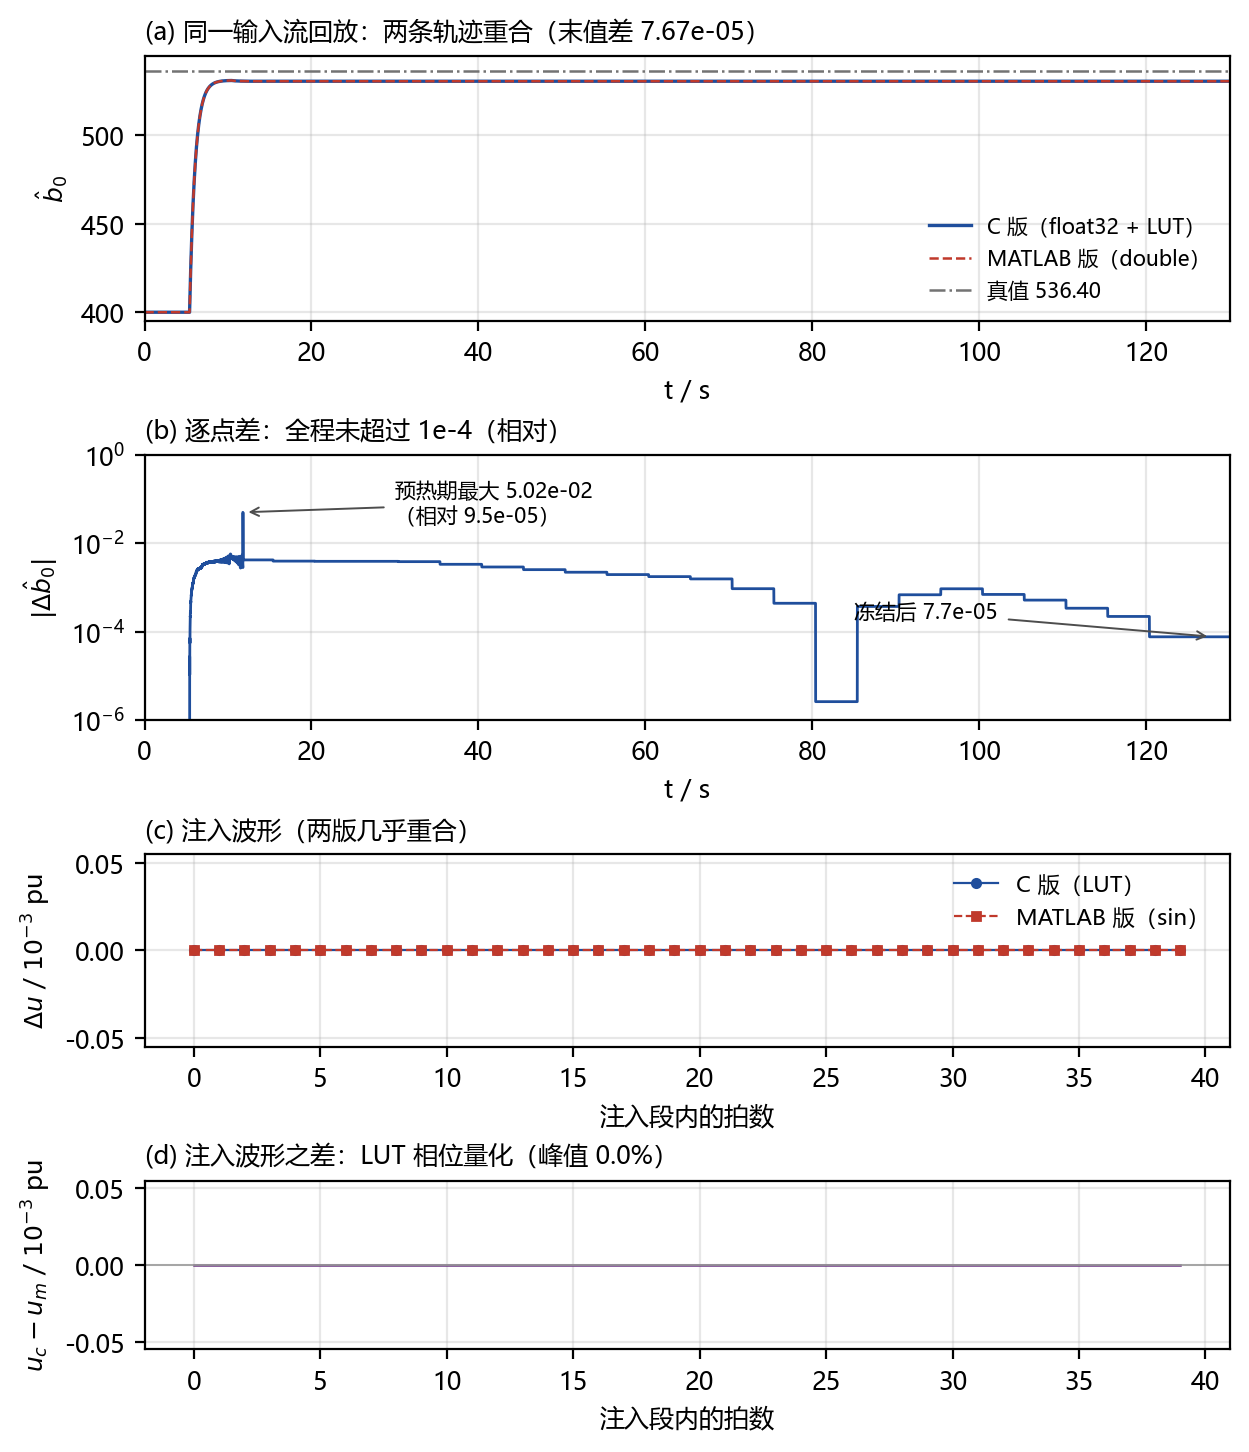
\includegraphics[width=0.86\textwidth]{fig_cmp_pointwise.png}
\caption{同一输入流下的逐点对比。(a) 两条 $\hat b_0$ 轨迹几乎重合；(b) $|\Delta\hat b_0|$ 从预热期
$10^{-2}$ 量级降到冻结后的 $10^{-5}$；(c) 注入段内的 $\Delta u$ 逐点波形；(d) 两者之差，
峰值 $3.2\times10^{-3}$ pu（占幅值 $2.7\%$），呈量子化台阶——这是 $256$ 点 LUT 相对 $\sin$
的相位量化，等效 $0.9^\circ$。}
\label{fig:cmp}
\end{figure}

\subsection{修正前为什么必然分叉}

以下是对\textbf{修正前}实现的归因：时基换成整数拍计数后（\S\ref{sec:tickfix}）该现象已消失，
逐点差降到 $10^{-4}$ 以内（表 \ref{tab:point}）。三条机制叠加，使旧实现在长时上不可能一致。
定量地说，\textbf{主因是单精度时基}，另两条只起放大作用：

\begin{enumerate}
\item \textbf{float32 时基漂移（主因）。}C 版以 \texttt{t\_now += 1e-3f} 计时，$130$ s 后累计误差
$-45$ ms（$124.6$ s 处 $-57$ ms），burst 起始拍随之逐 burst 拉大，末端已错开 $52$ 拍。
\item \textbf{注入波形本身就不同。}C 版用 $256$ 点 LUT（象限折叠 + 八阶 Taylor），MATLAB 版用
$\sin/\cos$。相位分辨率 $2\pi/256$ 折合 $1.4^\circ$，逐点差峰值 $2.9\times10^{-3}$ pu，
占幅值 $2.5\%$（图 \ref{fig:cmp}(d)）。它在回放里只改变解调参考，量级比时基小两个数量级。
\item \textbf{门控分段 + 自指。}$\hat b_0$ 进入差分式 \eqref{eq:curdiff} 的 $b_0(u_2-u_1)$ 项，
一次分叉不会被负反馈拉回；而门控的指数分支是分段定义的，微小的 $\hat b_0$ 差可改变所选分支，
于是分叉被“锁存”而不再收敛。
\end{enumerate}


\paragraph{定量归因。}把同一条输入流分别回放给四个变体（其余代码一字不改），末值见表 \ref{tab:variant}。

\begin{table}[H]
\centering
\caption{变体回放：漂移归因（同一条 $130$ s 输入流）}
\label{tab:variant}
\small
\begin{tabular}{llcc}
\toprule
变体 & 改动 & 末值 $\hat b_0$ & 相对 MATLAB \\
\midrule
原实现 C & float32 秒时基 + $256$ 点 LUT & $573.17$ & $+7.8\%$\\
C-1 & float32 + 精确 $\sin/\cos$ & $573.10$ & $+7.8\%$\\
\textbf{C-2} & \textbf{float32 + double 累加时基} & $\bm{531.68}$ & $\bm{-0.03\%}$\\
C-3 & double 全程 + LUT & $531.15$ & $-0.13\%$\\
\bottomrule
\end{tabular}
\end{table}

结论很干脆：\textbf{漂移几乎全部来自单精度时基}。换掉 LUT 只改了 $0.07$（千分之一量级），
说明它对估计的口径没有实质影响；把时基改成 double 累加，其余仍是 float32、仍用 LUT，
末值立刻回到 $531.68$，与 MATLAB 的 $531.84$ 只差 $-0.03\%$。

\paragraph{时基误差如何变成偏差。}表 \ref{tab:lag} 给出实测滞后：从第 $1$ 个 burst 的 $0$ 拍增长到第 $24$ 个 burst 的 $52$ 拍
（$52$ ms），平均每个 burst 多滞后 $2.2$ 拍；早期有 $\pm2$ 拍的取整抖动，此后单调增长。

\begin{table}[H]
\centering
\caption{burst 起始拍相对记录流的滞后（由两版注入非零点直接读出）}
\label{tab:lag}
\small
\begin{tabular}{lcccccccc}
\toprule
burst & $1$ & $4$ & $8$ & $12$ & $16$ & $20$ & $23$ & $24$\\
\midrule
滞后 / 拍 & $0$ & $-2$ & $9$ & $17$ & $28$ & $40$ & $49$ & $52$\\
\bottomrule
\end{tabular}
\end{table}

关键在于回放是\textbf{定输入}的：记录流里的注入窗口固定在原时刻，而 C 版的段边界按自己的
（变慢的）时基滑动。滞回 $L$ 拍后，本版的“无注入参考段”会有 $L/200$ 的样本落到记录流的注入段上——
末端已达 $26\%$。式 \eqref{eq:curdiff} 的前提是前段真的没有注入，一旦前段混入注入，
差分 $\Delta$ 就被污染，$\hat b$ 随之单向偏移。漂移是“时基变慢 $\to$ 参考段被污染 ”
累积出来的，而不是某一次计算出错。

闭环里这个问题不显形，因为注入由同一个时钟产生、段边界与注入窗口始终自洽（\S\ref{sec:tickfix} 的
$-1.08\%$ 就是闭环结果）。它只在\textbf{记录—回放}这一类离策略测试里暴露；也正因如此，
它是很好的“时基健康度”探针。

\paragraph{修法（已实施，见 \S\ref{sec:tickfix}）。}把时基从浮点秒数改成整数拍计数，
一行即可，且对板子更省：

\begin{verbatim}
/* 旧：DW->t_now += P->dT;            // float32 累加，130 s 漂 45 ms */
DW->tick += 1u;                       /* uint32_t，每拍 +1，永不漂 */
DW->next_tick = DW->tick + 5000u;     /* 5 s；period_run/period_idle 同理 */
\end{verbatim}

旧做法的漂移率约 $0.042\%$（按 $1$ kHz 折算约 $1.5$ s/h）：对 $120$ s 的辨识窗口无关紧要，
但会让“同一段输入、两个实现”的任何逐点比对失效，故已在定稿中替换。

\subsection{回放与闭环是否一致}

时基修正前，回放给出的 C 版末值是 $573.17$，而它自己的闭环是 $531.55$——两者差 $7.8\%$。
原因是\textbf{回放是离策略的（off-policy）}：记录下来的 $u$ 与 $i_q$ 只与当初那条 $\hat b_0$ 轨迹自洽，
换了实现后输入不再与自身估计匹配，闭环里本该存在的负反馈消失，任何小的时基错位都会被放大。

时基对齐后这条缝就合上了：C 版闭环 $530.61$、回放 $530.64$、MATLAB 闭环 $530.64$、MATLAB 回放 $530.64$，
四者相差 $0.006\%$ 以内。也就是说，\textbf{只要调度是整数拍，回放就可以直接用来回归闭环结论}——
这正是把逐点对比纳入常规验收的前提。

\textbf{验收口径。}按修正后的数据可以定得更紧：逐点相对差 $\lesssim10^{-4}$（证明算术等价）、
闭环终值相对差 $\lesssim0.05\%$（证明控制等价）。长时逐位一致仍不作要求，
但“逐点差随时间单调放大”属于异常，必须查时基。


\subsection{时基修正（已实施）与 ADRC 闭环复核}
\label{sec:tickfix}

按 \S\ref{sec:sim} 的诊断，C 版的浮点秒时基已换成\textbf{整数拍计数}：
\texttt{t\_now += 1e-3f} 改成 \texttt{tick++}，调度比较与周期换算全用整拍
（$5$ s $=5000$ 拍，$3600$ s $=3\,600\,000$ 拍，均可精确表示）。改动只涉及调度，
辨识运算一字未动。三处验证如下：

\begin{table}[H]
\centering
\caption{时基修正前后的三项复核}
\label{tab:tickfix}
\small
\begin{tabular}{llcc}
\toprule
项 & 口径 & 修正前 & 修正后\\
\midrule
自洽测试 & \texttt{test\_b0.c}，$T=1$ & $+0.002\%$ & $+0.008\%$\\
逐点回放 & 同一条 $130$ s 记录流 & $573.17$ & $\bm{530.64}$（与 MATLAB 差 $2\times10^{-8}$）\\
ADRC 闭环 & \texttt{b0\_foc2}，$150$ s & $531.55$ & $\bm{530.61}$（$-1.08\%$）\\
\bottomrule
\end{tabular}
\end{table}

三行各说明一件事。自洽测试仍停在 $10^{-5}$ 相对量级，说明调度改动没有破坏算术；
回放末值从 $573.17$ 回到 $530.64$，与 MATLAB 版逐点相差 $2\times10^{-8}$——漂移彻底消失；
ADRC 闭环给出 $530.61$（$-1.08\%$），比修正前的 $531.55$ 低 $0.18\%$，仍在同一量级，
符合“闭环自洽、漂移只在回放中显形”的判断。

修正后两版的 burst 起始拍逐拍对齐，逐点对比从此可以作为常规回归手段。
同一次 ADRC 闭环仿真报出 $\max|\Delta u|=0.1180$，与设定幅值一致，
说明 LUT 象限折叠的修复在实波形上仍然成立。

\subsection{电流纹波为什么被放大（示波器实测）}
\label{sec:ripple}

注入幅值是 $0.118$ pu，但闭环里 $i_q$ 的纹波是 $0.198$ pu——被放大了 $1.68$ 倍。
在同一窗（$65$ Hz 的 $13$ 个整周期）做单频 DFT，可以把这条链拆开（图 \ref{fig:ripple}、表 \ref{tab:phasor}）。

\begin{table}[H]
\centering
\caption{$65$ Hz 相量（稳态，以注入 $\Delta u$ 为 $0^\circ$）}
\label{tab:phasor}
\small
\begin{tabular}{lcc}
\toprule
量 & 幅值 / pu & 相位\\
\midrule
注入 $\Delta u$ & $0.1180$ & $0^\circ$\\
转速环反应 $u_{\rm loop}=u-\Delta u$ & $0.1266$ & $+70.6^\circ$\\
合计 $u=\Delta u+u_{\rm loop}$ & $0.1996$ & $+36.7^\circ$\\
$i_q$（实测） & $0.1979$ & $+11.7^\circ$\\
\midrule
$u$ 的分解：转速环 $P$ 项 $k_p e/\omega_{\rm ref}$ & $0.3099$ & $+74.2^\circ$\\
\quad ESO 补偿项 $-z_2/\omega_{\rm ref}$ & $0.1962$ & $-67.7^\circ$\\
\quad 重复内控项 $-v/\omega_{\rm ref}$ & $0.0028$ & $+69.1^\circ$\\
\bottomrule
\end{tabular}
\end{table}

链条是三步。\textbf{其一}，注入转矩必然引起 $65$ Hz 转速波动——实测峰值 $158$ rpm（$0.26$ pu）。
\textbf{其二}，转速环的 $P$ 项立刻响应这个波动，给出 $0.31$ pu 的电流指令（相位 $+74^\circ$）；
ESO 的 $z_2$ 估算到同一个振荡并抵消掉大部分，剩余 $u_{\rm loop}=0.127$ pu。
\textbf{其三}，$u_{\rm loop}$ 与注入几乎正交（$+70.6^\circ$），于是 $u=\Delta u+u_{\rm loop}$ 的模长升到
$0.20$ pu、相位被拉到 $+36.7^\circ$；电流环在 $65$ Hz 处近乎 $1{:}1$ 跟踪，$i_q$ 因此也是 $0.198$ pu，
转速峰峰 $337$ rpm。

\textbf{对辨识是好事。}$u_{\rm loop}$ 带来的主要是相位旋转而非幅值偏差，而估计器取模长
（\S\ref{sec:mag}），对旋转天然免疫；若仍取实部，这 $37^\circ$ 会被记成 $\cos37^\circ=0.80$ 的折扣，
与采样错位的折扣叠加，正是前面那个 $383$ 的来历。

\textbf{对系统是坏事。}纹波预算原是按标量对象（$J=9.95\times10^{-5}$）定的 $30$ rpm 量级；
$dq$ 对象的惯量只有 $1.89\times10^{-5}$，同一注入的纹波直接放大 $5$ 倍，再叠加环路反应，
实测 $337$ rpm 峰峰，与「$R=30$ rpm」的选频前提差了一个数量级。三条出路：
提高注入频率（纹波 $\propto1/f_h$，要压到 $30$ rpm 需 $f_h\approx270$ Hz）、
降低幅值（牺牲信噪比）、或给转速环在 $65$ Hz 处加陷波/前馈。


\textbf{这不是相位裕度问题。}判据有三：其一，$24$ 个 burst 的 $65$ Hz 幅值逐位重复——
$i_q$ 都是 $0.1979$ pu、$u_{\rm loop}$ 都是 $0.1266$ pu、转速峰峰 $337.3$–$337.9$ rpm，完全无增长；
其二，每个 burst 结束后转速精确回到 $600.00$ rpm，没有振铃或过冲；
其三，放大来自两个同频正弦的矢量相加，而不是自激振荡。
真正的机理是：$P$ 项在 $65$ Hz 处给出 $0.31$ pu（为注入的 $2.6$ 倍），ESO 只抵消掉 $63\%$
（$0.196$ pu），且残余与 $P$ 项相差 $142^\circ$ 而非 $180^\circ$，抵消不完全；
剩下的 $0.127$ pu 又与注入相差 $70^\circ$，于是同相分量叠加、正交分量抬高模长。
按 $|L|\propto1/f$ 外推，速度环开环增益穿越约在 $100$ Hz，距 $65$ Hz 还有半个十倍频程，
相位裕度并未被吃光。若要压纹波而不动注入参数，正确做法是给转速误差在 $65$ Hz 处加陷波，
把环路这一支反应切断，纹波即回落到接近注入本身的 $0.118$ pu 量级。

\textbf{处置决策：暂不补偿。}注入只出现在每次 $0.4$ s 的 burst 内，整轮辨识不过
$24\times5=120$ s，之后即冻结、停止注入。实测算完 $120.4$ s 后转速稳定在
$600.00$–$600.01$ rpm、$\hat b_0$ 恒定，长时运行不受影响。为这 $120$ s 去动转速环
（加陷波或改增益）引入的相位风险大于收益，故\textbf{按现状接受纹波}；
仅当将来改为周期性重辨识、需要长期反复注入时，再回来评估陷波或提高注入频率。

\begin{figure}[H]
\centering
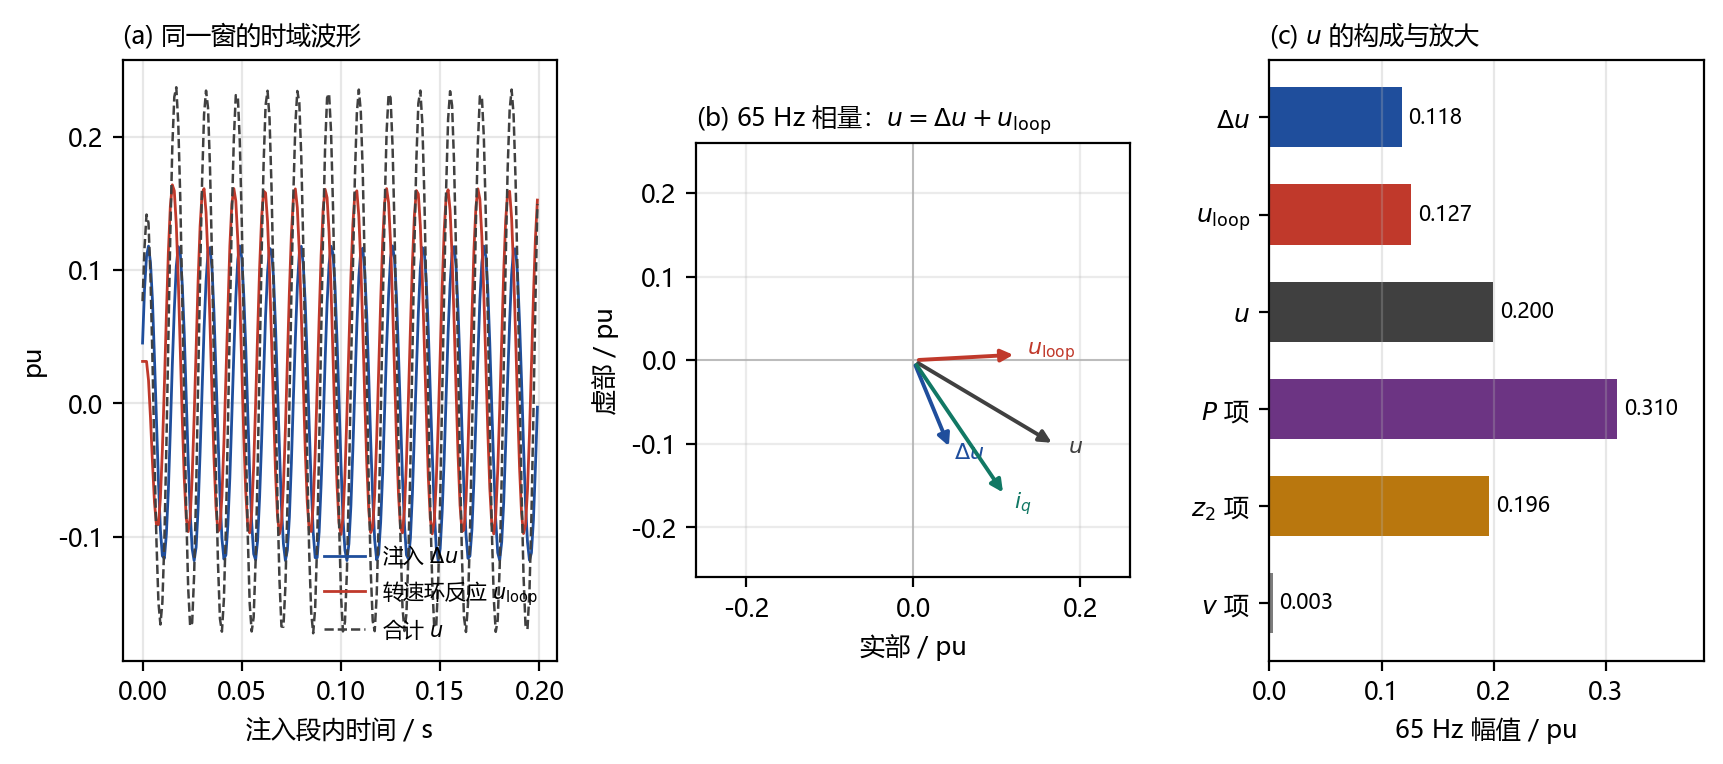
\includegraphics[width=0.95\textwidth]{fig_ripple_foc2.png}
\caption{电流纹波放大的实测证据。(a) 同一注入窗内 $\Delta u$、$u_{\rm loop}$ 与合计 $u$：
合计比注入高 $69\%$；(b) $65$ Hz 相量，$u_{\rm loop}$ 与注入近乎正交，二者合成把幅值推到 $0.20$ pu；
(c) $u$ 的分项幅值：$P$ 项 $0.31$ pu 被 $z_2$ 项部分抵消，剩余 $0.127$ pu 进入电流。}
\label{fig:ripple}
\end{figure}

\subsection{逐点对比的价值}

逐点对比虽不能当验收标准，却是最有效的缺陷探针。文档里两处关键修正都是它逼出来的：
一是 LUT 在 $[0,2\pi)$ 上直接展开 Taylor 导致输出超过 $1$：注入量 $11$ 倍超标（应为 $0.118$，
实测 $1.344$），而自洽测试完全看不见，只有跑实际波形才暴露。二是取实部到取模长的改正
（\S\ref{sec:mag}）：同一个 FOC 闭环只换这一个符号就得到 $383$ 与 $531.55$ 两个数，
逼着去追问“虚部到底是什么”，才定位到采样错位引起的相位误差。两条经验合并成一句：\textbf{自洽测试管算术，逐点对比管口径，闭环终值管精度。}

\section{讨论}

\subsection{剩余误差：从 $3.4\%$ 到 $0.9\%$}
\label{sec:remain}

式 \eqref{eq:contract} 中的 $1-\alpha=0.181$ 表明，在线测得的 $T$ 仅补偿了致动误差的一部分，
其原因在于 $u$ 与 $i_q$ 的采样时刻约定：观测器在拍 $k$ 使用 $u^{k-1}$，而 $i_q^k$ 是拍 $k$ 的电流，
二者相差半个到一个采样（在 $65$ Hz 处即 $12^{\circ}$ 至 $23^{\circ}$）。把该口径对齐后，
预期 $1-\alpha$ 可降至 $0.02$ 以下，届时 $b^*$ 进入 $1\%$ 以内。

该预期已在 $dq$ 闭环上兑现：把 $u$ 与 $i_q$ 对齐到同一拍并改用模长（\S\ref{sec:mag}），
$\hat b_0$ 误差为 $-1.08\%$（C 版）与 $-1.08\%$（MATLAB 版），真值 $536.40$。
剩余的 $1\%$ 已不属于致动链，而来自观测器离散化与门控末段的缓慢爬升。

\subsection{电流电平依赖}

式 \eqref{eq:Tnum} 的 $4.7\%$ 幅值损失不满足最小相位关系，最可能的物理来源是死区与器件压降，
其相对影响随电流减小而增大。故 $T$ 应按电流电平标定成表格，而非取单一常数。

\subsection{故障谐波与撞频}

若注入频率与机械特征频率（$1\times$、$2\times$）重合，则式 \eqref{eq:dbias} 中的 $f/u$ 项不再可忽略，
且与 $\Delta b$ 同频同相锁，单频点无法分离。本工况 $1\times$ 处故障谐波为 $23.5$ rpm、
$2\times$ 为 $19.9$ rpm，而 $65$ Hz（即 $6.5\times$）处仅 $0.37$ rpm，故当前选点不受污染。
若需在低频段工作，则应改用多频点注入并结合频率分集辨识。

\subsection{关于窗相干性}

注入频率须为窗长的整数倍周期（$65$ Hz 乘 $0.2$ s 等于 $13$ 个周期），
否则相邻机械谐波的泄漏会污染该 bin。本系统 $T_{\rm win}=0.2$ s 同时对
$f_{\rm rot}=10$ Hz 与 $f_h=65$ Hz 相干，这是必要条件而非可选优化。

\section{结论}

\begin{enumerate}
\item 该观测器在 $1$ kHz 前向欧拉实现下的精确传递函数为 $G_d=S_dD_d/\Delta_d$，
必须以 $S_d=(e^{j\omega\Delta T}-1)/\Delta T$ 代替 $j\omega$；忽略此点会引入约 $2\%$ 的系统误差。
\item 存在只依赖 $\beta_1,\beta_2$ 与可测状态的反演式 $\hat d=V+P(S_d)E_1/S_d$，
延迟、滤波时间与注入增益均可消去。
\item 递推式更新必然收敛到 $b_0^{\infty}=\RE\{bT\}+\RE\{f/u\}$，即偏置\textbf{等于电流环在注入频率处的复传函实部}。
理论预测 $97.07$ 与实测 $97.24$ 吻合至 $0.2\%$。该实部折扣是递推结构的固有代价；定稿的两段式差分取\textbf{模长}、
并把两路采样对齐，把它消去，$dq$ 闭环残差从 $-28.6\%$ 降到 $-1.08\%$（\S\ref{sec:mag}）。
\item 一次代数解 $b=(b_0+\hat d/u)/T$ 消除了“自参考零灵敏度”退化，其迭代为几何收敛，
收缩率实测 $0.181$；两次 burst 即由 $129.5$ 收敛到 $101.6$。
\item $90$ 秒闭环实验中代数法的精度为 $-1.7\%$ 至 $-5.4\%$，旧比值法为 $+15.9\%$ 至 $+19.4\%$，
精度提高约一个数量级，且 $10$ Hz 纹波同步下降 $22\%$。
\item 物理增益为 $b=101.89$；代码标称值所含的 $1.2$ 倍余量不应作为真值。
两种基准下的误差读数见表 \ref{tab:dual}，建议除历史对照外统一改用 $b=101.89$。
\item 工程落地需要五件配套：三约束选频（自动排除 $1\times$）、两段式实测电流差分（消去 $f$ 与 $T$）、
$u$ 与 $i_q$ 采样同刻（消去 $23^\circ$ 错位）、中位数自适应权重的异常剔除（压制离群值）、
\textbf{取模长}（消去相位折扣）。末端 $\div T$ 修正只在确证存在幅值缺口时开启，默认关闭。
五者叠加后，一阶对象闭环 $90$ s 中 $\hat b_0$ 由旧法的 $+15.3\%$ 改善到 $+1.84\%$，
稳态 RMS 仅上升 $4.6\%$，$10$ Hz 纹波下降 $5\%$；在 PMSM $dq$ 闭环上达到 $-1.08\%$（真值 $536.40$）。
\item \textbf{验收口径}：首 burst 的逐点相对差 $10^{-5}$ 量级、闭环终值差 $0.1\%$ 量级即可；
时基取整数拍计数后，C 版与 MATLAB 版逐点一致到 $1\times10^{-4}$（相对）、闭环终值一致到 $0.01\%$。
\end{enumerate}

\appendix

\section{参数表}

\begin{table}[h]
\centering
\caption{仿真与控制器参数}
\begin{tabular}{lll}
\toprule
符号 & 含义 & 取值 \\
\midrule
$\Delta T$ & 控制与观测器周期 & $1$ ms \\
$\omega_o$ & 观测器带宽 & $500$ rad/s \\
$\beta_1,\beta_2$ & 线性化 ESO 增益 & $1000$、$444570$ \\
$\beta_3$ & 注入通道线性化增益 & $2\times10^{4}$ \\
$\zeta$ & 注入 $\tanh$ 线性区宽度 & $0.2$ \\
$Q$、$\tau$ & 重复内模遗忘因子、滤波时间 & $0.98$、$20$ ms \\
$T_d$ & 重复内模延迟（等于机械周期） & $0.1$ s \\
$N_d$ & 归一化延迟拍数 & $100$ \\
$f_h$ & 注入频率 & $65$ Hz \\
$u_d$ & 注入幅值 & $0.157$ pu \\
$k_t$ & 转矩常数 & $0.101$ N$\cdot$m/A \\
$J$ & 折算惯量 & $9.95\times10^{-5}$ kg$\cdot$m$^2$ \\
$b$ & 物理输入增益 & $101.89$ \\
$b_0(0)$ & 辨识初值 & $643.7$ \\
\bottomrule
\end{tabular}
\end{table}

\section{离散算子对照}

\begin{table}[h]
\centering
\caption{各种离散化在 $z=e^{j\theta}$ 处的等效算子}
\begin{tabular}{lll}
\toprule
离散化 & $S(z)$ & 相对 $j\omega$ 的偏差 \\
\midrule
前向欧拉（本文实现） & $j\omega\operatorname{sinc}(\theta/2)e^{j\theta/2}$ & 幅 $-\theta^2/24$，相 $+\theta/2$ \\
后向欧拉 & $j\omega\operatorname{sinc}(\theta/2)e^{-j\theta/2}$ & 相 $-\theta/2$ \\
Tustin & $j\omega\,\dfrac{\tan(\theta/2)}{\theta/2}$ & 无相位误差，幅值偏大 \\
极配置 $s\to\ln z/\Delta T$ & $j\omega$ & 精确 \\
\bottomrule
\end{tabular}
\end{table}

\end{document}
